%appendix
\chapter{Supplementary Material} \label{sec:appendix}

This chapter contains supplementary material for additional insight, as well as plots that provide more qualitative information.
In addition, some tables are included here that provide more detailed insights into the data compilation process.
Everything is arranged chronologically according to occurrence in the main section and shares the headline of each chapter for easy reference.

\section{Sources}

\begin{table}
  \centering
  \caption{Table of the first half of the $\num{72}$ GFU-gold events used as sources in this analysis. Shown are the features time in MJD, declination $\delta$ in degrees, right ascension $\alpha$ also in degrees and signalness in percent. The time-dependent analysis uses a subset of these sources highlighted in red. The order of the sources corresponds to the processing order in the analysis pipeline.}
  \label{tab:sources_v2}
  \begin{tabular}{ccrrc}
    \toprule
    Nr. & MJD &  $\delta$ in $\si{\degree}$ & $\alpha$ in $\si{\degree}$ & signalness in $\si{\percent}$ \\
    \toprule
      1 & 55695.06 & -1.94 & 138.47 & 50.80 \\ 2 & 57709.33 & 1.60 & 78.66 & 50.40 \\ 3 & 57284.21 & 30.35 & 279.54 & 67.40 \\ 4 & 58806.04 & 3.77 & 229.31 & 45.10 \\ 5 & 56927.16 & -0.63 & 50.89 & 48.10 \\ 6 & 55722.43 & 35.64 & 272.55 & 75.00 \\ 7 & 57938.29 & 23.36 & 230.45 & 60.20 \\ 8 & 59204.53 & 41.81 & 261.69 & 56.40 \\ 9 & 57758.14 & 8.16 & 309.95 & 53.50 \\ 10 & 57157.94 & 12.14 & 91.49 & 76.80 \\ \textcolor{red}{11} & \textcolor{red}{56819.20} & \textcolor{red}{11.45} & \textcolor{red}{110.65} & \textcolor{red}{99.70} \\ \textcolor{red}{12} & \textcolor{red}{56470.11} & \textcolor{red}{14.17} & \textcolor{red}{93.74} & \textcolor{red}{93.80} \\ \textcolor{red}{13} & \textcolor{red}{57951.82} & \textcolor{red}{25.16} & \textcolor{red}{208.39} & \textcolor{red}{86.60} \\ 14 & 58618.45 & 12.60 & 127.88 & 81.60 \\ 15 & 57974.60 & -2.28 & 21.27 & 59.80 \\ \textcolor{red}{16} & \textcolor{red}{58063.78} & \textcolor{red}{7.44} & \textcolor{red}{340.14} & \textcolor{red}{97.50} \\ 17 & 57443.88 & 60.06 & 311.87 & 59.60 \\ 18 & 57662.44 & 37.12 & 192.57 & 63.90 \\ 19 & 58653.55 & 10.28 & 343.52 & 54.70 \\ 20 & 57887.30 & 30.65 & 227.37 & 55.30 \\ 21 & 59121.74 & 3.47 & 29.53 & 47.50 \\ 22 & 57391.44 & 5.00 & 79.41 & 56.60 \\ 23 & 58225.28 & -4.41 & 305.73 & 57.70 \\ 24 & 57269.76 & 28.08 & 133.77 & 74.10 \\ 25 & 56843.67 & 2.54 & 25.88 & 55.90 \\ 26 & 56579.91 & 10.28 & 32.92 & 66.50 \\ 27 & 57989.55 & 12.37 & 41.92 & 48.90 \\ 28 & 58019.02 & -2.54 & 173.45 & 56.30 \\ \textcolor{red}{29} & \textcolor{red}{57340.87} & \textcolor{red}{12.71} & \textcolor{red}{76.16} & \textcolor{red}{95.70} \\ 30 & 58857.99 & 11.80 & 165.45 & 76.90 \\ 31 & 56062.96 & 32.00 & 198.94 & 61.30 \\ 32 & 56817.64 & 1.31 & 106.26 & 81.50 \\ 33 & 58647.83 & 26.57 & 312.19 & 60.60 \\ 34 & 56146.21 & 1.42 & 330.07 & 74.40 \\ 35 & 58141.68 & 8.01 & 77.12 & 78.80 \\ 36 & 57655.74 & 1.34 & 241.13 & 50.80 \\ 
    \toprule
  \end{tabular}
\end{table}

\begin{table}
  \centering
  \caption{Table of the second half of the $\num{72}$ GFU-gold events used as sources in this analysis. Shown are the features time in MJD, declination $\delta$ in degrees, right ascension $\alpha$ also in degrees and signalness in percent. The time-dependent analysis uses a subset of these sources highlighted in red. The order of the sources corresponds to the processing order in the analysis pipeline.}
  \label{tab:sources_v2_2}
  \begin{tabular}{ccrrc}
    \toprule
    Nr. & MJD &  $\delta$ in $\si{\degree}$ & $\alpha$ in $\si{\degree}$ & signalness in $\si{\percent}$ \\
    \toprule
      \textcolor{red}{37} & \textcolor{red}{55911.28} & \textcolor{red}{18.88} & \textcolor{red}{36.74} & \textcolor{red}{94.60} \\ 38 & 57673.61 & -7.48 & 190.06 & 25.20 \\ 39 & 59168.09 & 1.38 & 195.12 & 46.00 \\ 40 & 59205.04 & 13.44 & 206.37 & 53.40 \\ 41 & 58442.71 & 11.72 & 25.71 & 53.70 \\ \textcolor{red}{42} & \textcolor{red}{56226.60} & \textcolor{red}{27.91} & \textcolor{red}{169.80} & \textcolor{red}{92.60} \\ \textcolor{red}{43} & \textcolor{red}{56666.50} & \textcolor{red}{33.02} & \textcolor{red}{293.12} & \textcolor{red}{92.70} \\ 44 & 57049.48 & 4.59 & 100.37 & 66.10 \\ 45 & 56620.15 & 19.47 & 285.16 & 55.30 \\ 46 & 58218.78 & 0.56 & 218.50 & 60.00 \\ 47 & 56757.10 & 81.22 & 2.11 & 62.70 \\ 48 & 58528.67 & -4.14 & 228.25 & 73.80 \\ 49 & 56319.28 & -1.98 & 352.97 & 61.00 \\ 50 & 57217.91 & 26.36 & 326.29 & 84.10 \\ 51 & 57312.68 & 19.95 & 197.53 & 75.40 \\ 52 & 58443.58 & 32.93 & 132.19 & 64.50 \\ 53 & 56658.40 & -2.69 & 192.26 & 56.00 \\ 54 & 59015.62 & 3.66 & 142.95 & 82.80 \\ 55 & 57246.76 & 6.17 & 328.27 & 83.10 \\ 56 & 57606.51 & -0.71 & 122.78 & 57.80 \\ 57 & 55811.79 & 9.40 & 196.08 & 50.60 \\ \textcolor{red}{58} & \textcolor{red}{57478.57} & \textcolor{red}{15.48} & \textcolor{red}{151.22} & \textcolor{red}{85.10} \\ 59 & 58018.87 & 5.79 & 77.43 & 63.10 \\ 60 & 58748.96 & -1.53 & 5.71 & 50.40 \\ 61 & 58757.84 & 12.79 & 313.99 & 59.00 \\ 62 & 57265.22 & 34.00 & 54.76 & 57.90 \\ \textcolor{red}{63} & \textcolor{red}{56211.77} & \textcolor{red}{-2.28} & \textcolor{red}{205.14} & \textcolor{red}{84.20} \\ 64 & 58694.87 & 10.77 & 226.14 & 67.00 \\ 65 & 57968.08 & 4.63 & 1.10 & 56.10 \\ 66 & 57930.52 & 8.80 & 280.99 & 54.70 \\ 67 & 55987.81 & 18.76 & 237.96 & 82.50 \\ 68 & 59167.63 & 5.87 & 105.73 & 56.20 \\ 69 & 59129.92 & 5.34 & 265.17 & 88.50 \\ 70 & 56186.31 & 3.88 & 182.24 & 43.80 \\ 71 & 57348.53 & -2.24 & 262.05 & 63.70 \\ 72 & 55806.09 & 7.59 & 9.76 & 60.90 \\ 
    \toprule
  \end{tabular}
\end{table}

%\begin{table}
%  \centering
%  \caption{Table of the sources used in the time-dependent analysis. Additionally the signalness parameter is shown after which the sources were selected.}
%  \label{tab:sources_time_dep}
%  \begin{tabular}{ccrrc}
%    \toprule
%    Nr. & MJD &  $\delta$ in $\si{\degree}$ & $\alpha$ in $\si{\degree}$ & signalness in $\si{\percent}$ \\
%    \toprule
%      11 & 56819.20 & 11.45 & 110.65 & 99.70 \\ 12 & 56470.11 & 14.17 & 93.74 & 93.80 \\ 13 & 57951.82 & 25.16 & 208.39 & 86.60 \\ 16 & 58063.78 & 7.44 & 340.14 & 97.50 \\ 29 & 57340.87 & 12.71 & 76.16 & 95.70 \\ 37 & 55911.28 & 18.88 & 36.74 & 94.60 \\ 42 & 56226.60 & 27.91 & 169.80 & 92.60 \\ 43 & 56666.50 & 33.02 & 293.12 & 92.70 \\ 58 & 57478.57 & 15.48 & 151.22 & 85.10 \\ 63 & 56211.77 & -2.28 & 205.14 & 84.20 \\ 
%    \toprule
%  \end{tabular}
%\end{table}

\section{Time-Integrated Search}

\begin{table}
  \centering
  \caption{Table of the number of injected signal events used for the time-integrated analysis.}
  \label{tab:sig_time_int_table}
  \begin{tabular}{r}
    \toprule
    $n_\text{S}$ injected \\
    \toprule
      0.0 \\ 7.5 \\ 15.0 \\ 22.5 \\ 30.0 \\ 36.0 \\ 57.0 \\ 78.0 \\ 99.0 \\ 120.0 \\ 141.0 \\ 194.2 \\ 247.4 \\ 300.7 \\ 353.9 \\ 407.1 \\ 460.3 \\ 513.6 \\ 566.8 \\ 620.0 \\ 
    \toprule
  \end{tabular}
\end{table}

\begin{table}
  \caption{Table of the number of trials for each spectral index $\gamma$ and number of injected signal events $n_\text{sig}$, running $\num{10}$ jobs with $\num{5e3}$ trials per set of parameter pairs $\gamma$ and $n_\text{sig}$. Some jobs fail due to technical reasons.}
  \label{tab:trials_sig_time_int_table}
  \begin{subtable}{\linewidth}
  \centering
  \begin{tabular}{p{.9cm}|rrrrrrrrrr}
    \toprule
    \: $n_\text{sig}$ \newline $\gamma$ \: & 0.0 & 7.5 & 15.0 & 22.5 & 30.0 & 36.0 & 57.0 & 78.0 & 99.0 & 141.0 \\ 
    \toprule
    1.50 & 50000 & 50000 & 50000 & 50000 & 50000 & 50000 & 50000 & 50000 & 50000 & 50000 \\ 1.75 & 50000 & 50000 & 50000 & 50000 & 50000 & 50000 & 50000 & 50000 & 50000 & 50000 \\ 2.00 & 50000 & 50000 & 50000 & 50000 & 50000 & 50000 & 50000 & 50000 & 50000 & 50000 \\ 2.25 & 50000 & 45000 & 45000 & 45000 & 50000 & 45000 & 50000 & 50000 & 50000 & 50000 \\ 2.50 & 50000 & 50000 & 50000 & 50000 & 50000 & 50000 & 50000 & 50000 & 50000 & 50000 \\ 2.75 & 50000 & 50000 & 45000 & 45000 & 50000 & 50000 & 50000 & 40000 & 50000 & 40000 \\ 3.00 & 50000 & 50000 & 50000 & 50000 & 50000 & 45000 & 50000 & 50000 & 50000 & 50000 \\ 
    \toprule
  \end{tabular}
\end{subtable}
\begin{subtable}{\linewidth}
\centering
  \begin{tabular}{p{.9cm}|rrrrrrrrrr}
    \toprule
    \: $n_\text{sig}$ \newline $\gamma$ \: & 141.0 & 194.2 & 247.4 & 300.7 & 353.9 & 407.1 & 460.3 & 513.6 & 566.8 & 620.0 \\ 
    \toprule
    1.50 & 50000 & 50000 & 50000 & 50000 & 50000 & 50000 & 50000 & 50000 & 50000 & 50000 \\ 1.75 & 50000 & 50000 & 50000 & 50000 & 50000 & 50000 & 50000 & 50000 & 50000 & 45000 \\ 2.00 & 50000 & 50000 & 50000 & 50000 & 50000 & 50000 & 50000 & 50000 & 50000 & 50000 \\ 2.25 & 50000 & 50000 & 50000 & 50000 & 50000 & 50000 & 50000 & 50000 & 50000 & 50000 \\ 2.50 & 50000 & 50000 & 50000 & 50000 & 50000 & 50000 & 50000 & 50000 & 50000 & 40000 \\ 2.75 & 50000 & 50000 & 50000 & 50000 & 50000 & 50000 & 50000 & 50000 & 50000 & 50000 \\ 3.00 & 50000 & 50000 & 45000 & 50000 & 50000 & 50000 & 50000 & 50000 & 50000 & 50000 \\ 
    \toprule
  \end{tabular}
  \end{subtable}
\end{table}

\section{Time-Dependent Search} \label{sec:time_dep_search_appendix}

In this chapter, the complete results for all $\num{10}$ sources can be found.

\subsection{Background Trials}

\begin{figure}
    \centering
    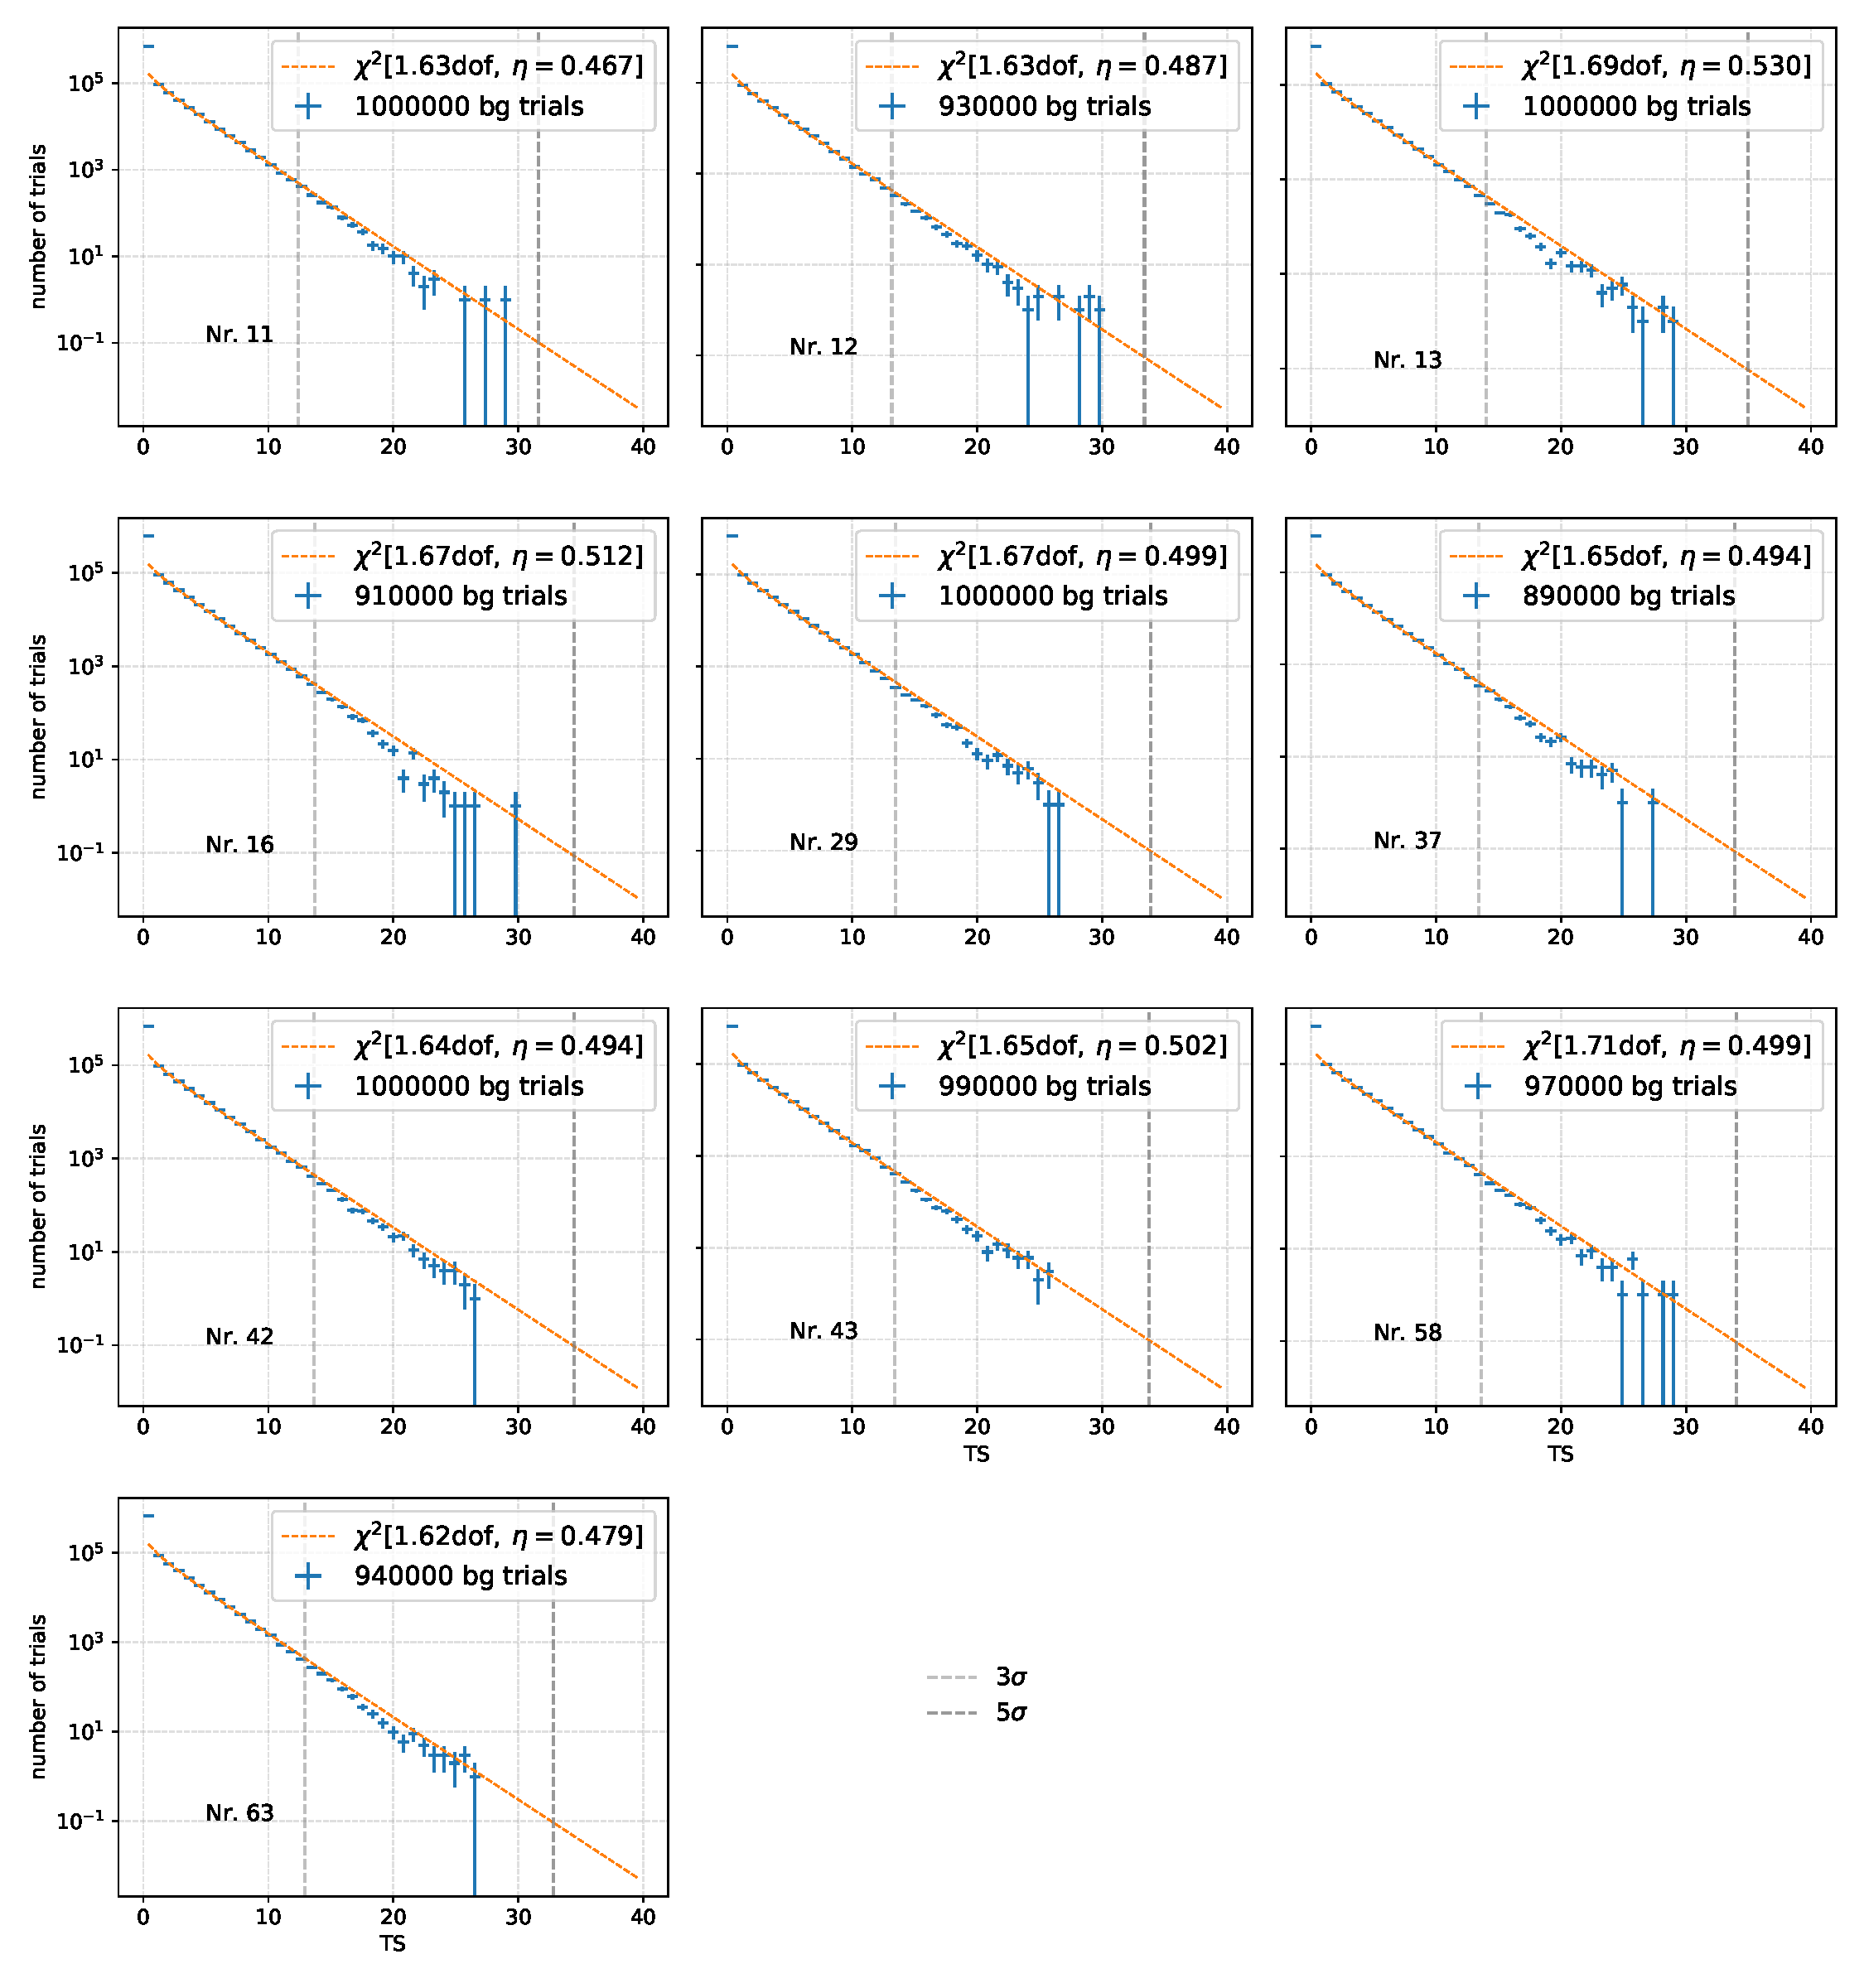
\includegraphics[width=\linewidth-2cm]{Plots/05_csky/9_years_gfu_gold_time_dep_bg_t0.pdf}
    \caption{Histograms of the background test statistic values for all $\num{10}$ sources used in the time-dependent analysis. Shown are also the number of degrees of freedom $dof$ and the ratio of positive and negative values $\eta$. The id of the sources corresponds to the tables \ref{tab:sources_v2} and \ref{tab:sources_v2_2}.}
    \label{fig:bg_trials_time_dep}
\end{figure}

\begin{figure}
    \centering
    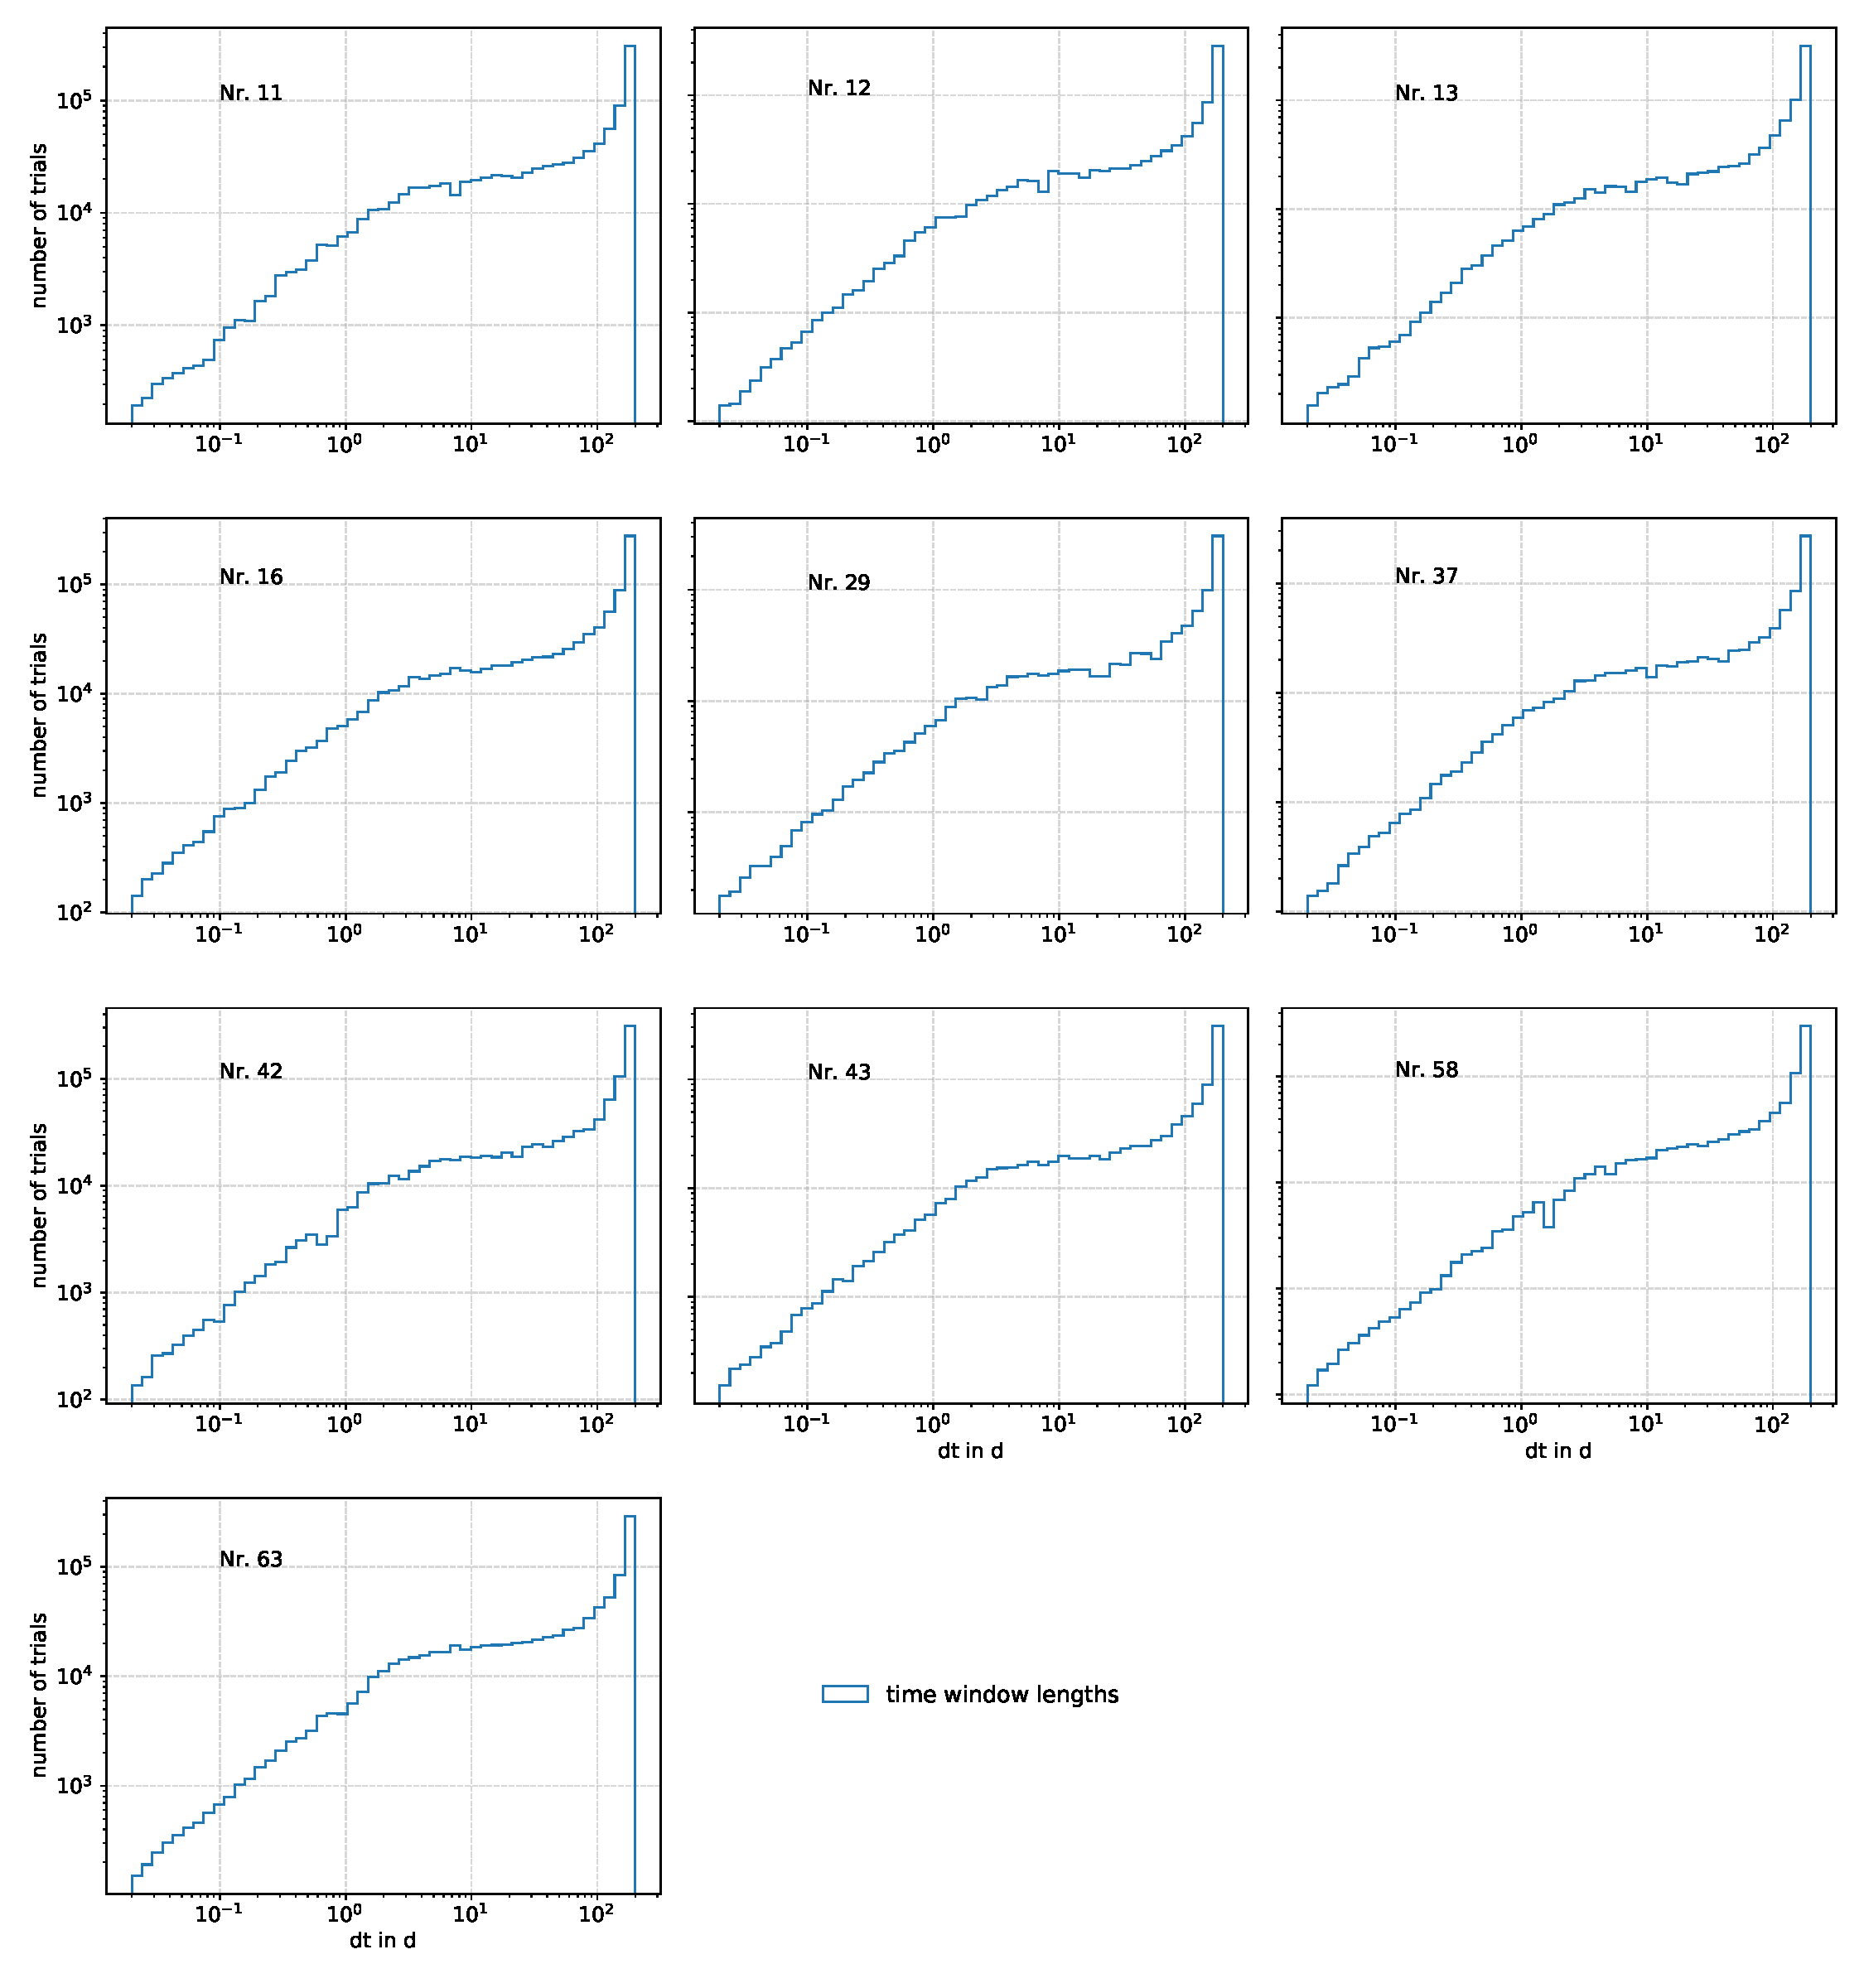
\includegraphics[width=\linewidth]{Plots/05_csky/9_years_gfu_gold_time_dep_bg_dt.pdf}
    \caption{Histograms of the background time window lengths $dt$ in days of all $\num{10}$ sources for the time-dependent analysis.}
    \label{fig:bg_trials_time_dep_time_windows}
\end{figure}

\begin{figure}
    \centering
    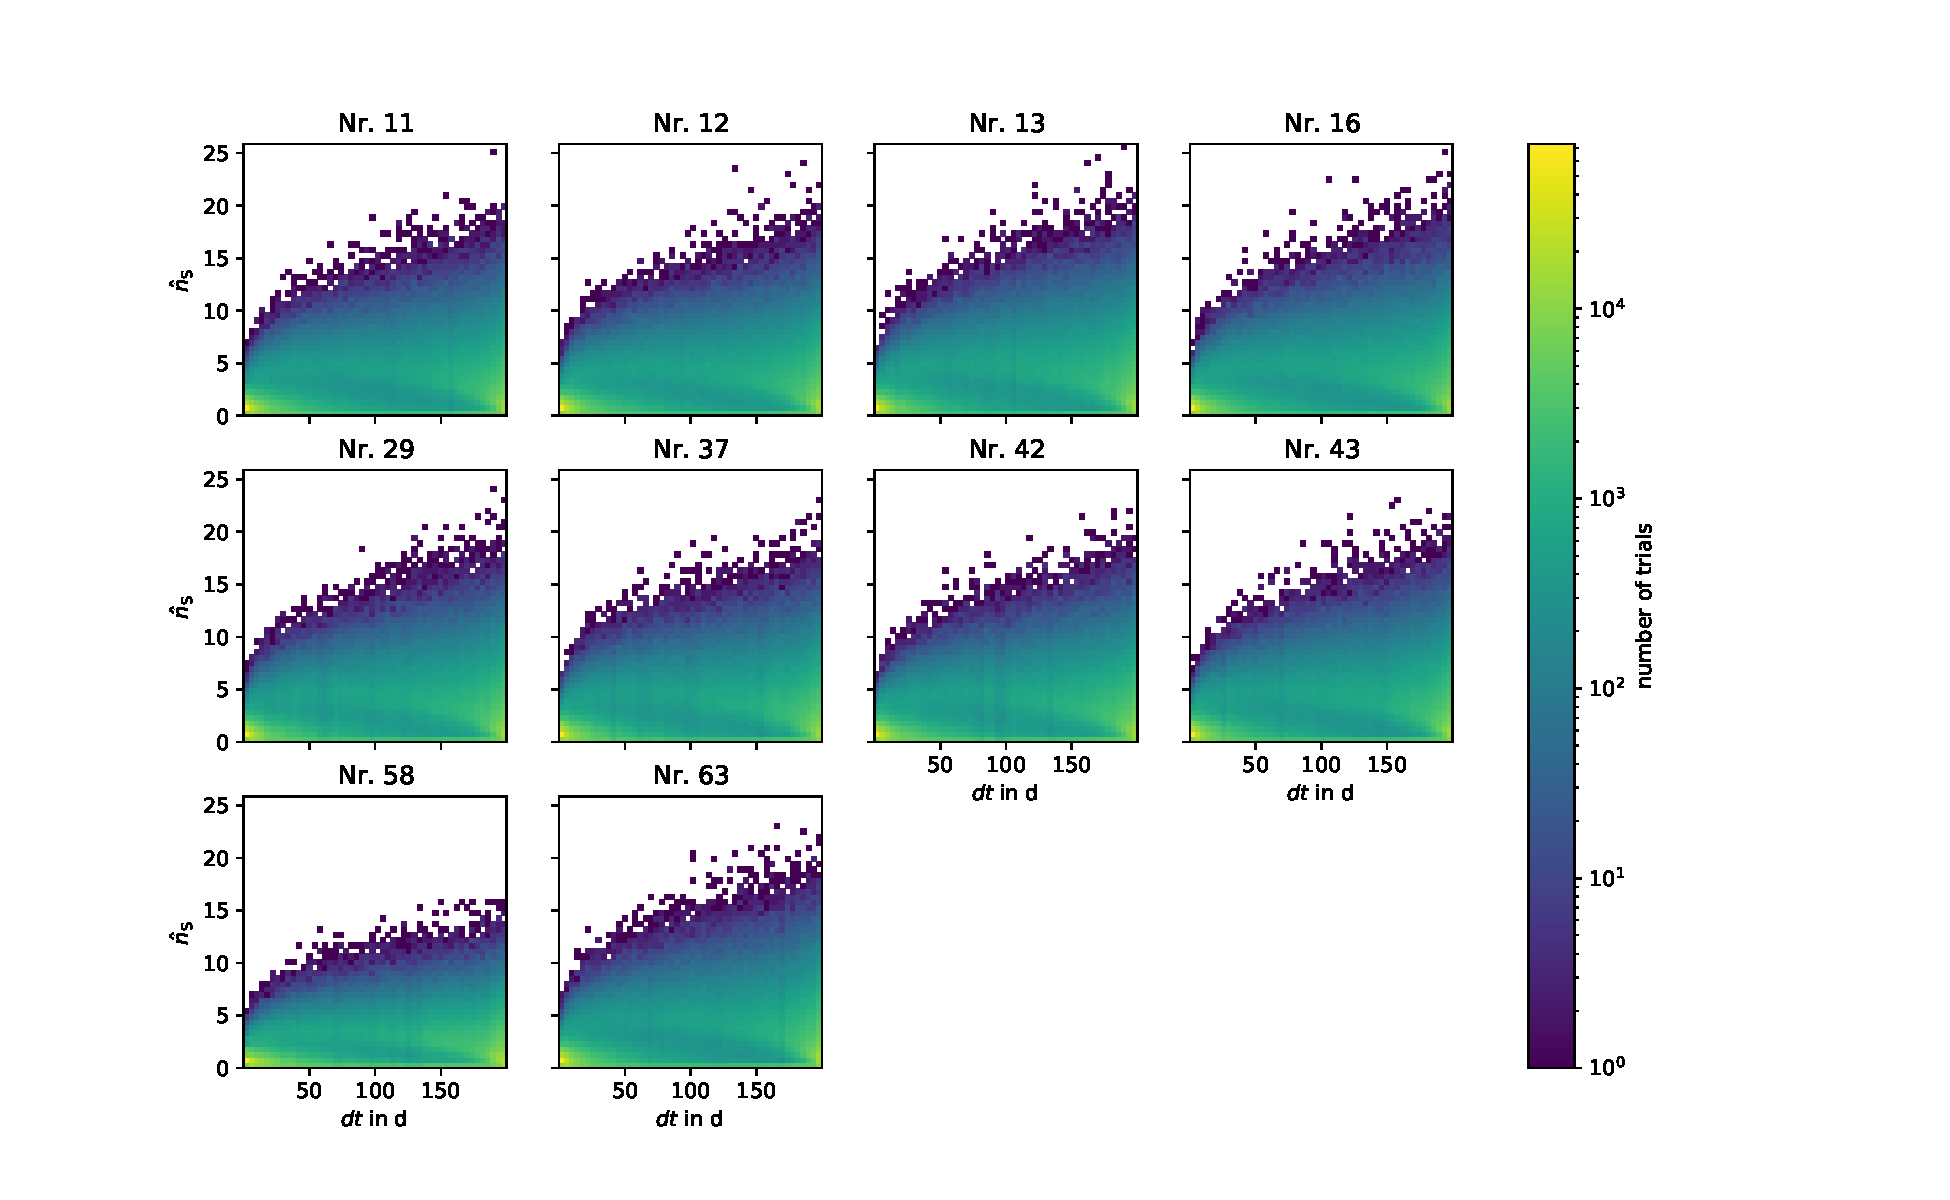
\includegraphics[width=\linewidth]{Plots/05_csky/time_window_ns_bg_time_dep.pdf}
    \caption{Histograms of the fitted number of signal events $\hat{n}_\text{S}$ in dependence of the time window lengths $dt$ in days of the background trials for the time-dependent analysis for all $\num{10}$ sources.}
    \label{fig:bg_trials_time_dep_time_windows_ns}
\end{figure}

\newpage
\subsection{Signal Trials}

\begin{table}
  \centering
  \caption{Table of the number of trials for each source index and number of injected signal events $n_\text{sig}$, running $\num{5}$ jobs with $\num{e4}$ trials per set of parameter pairs of source and $n_\text{sig}$. Some jobs fail due to technical reasons.}
  \label{tab:trials_sig_time_dep_table}
  \begin{tabular}{>{\centering\arraybackslash}p{.9cm}|%
                    cccccccccc}
    \toprule
    \: Nr. \newline $n_\text{sig}$ \: & 11 & 12 & 13 & 16 & 29 & 37 & 42 & 43 & 58 & 63 \\ 
    \toprule
    0.0 & 50000 & 50000 & 50000 & 50000 & 50000 & 10000 & 40000 & 50000 & 50000 & 30000 \\ 1.1 & 50000 & 50000 & 50000 & 50000 & 50000 & 20000 & 40000 & 50000 & 50000 & 20000 \\ 2.2 & 50000 & 50000 & 50000 & 50000 & 50000 & 0 & 40000 & 50000 & 50000 & 30000 \\ 3.3 & 50000 & 50000 & 40000 & 50000 & 50000 & 50000 & 40000 & 50000 & 50000 & 30000 \\ 4.4 & 50000 & 50000 & 30000 & 50000 & 50000 & 40000 & 50000 & 50000 & 50000 & 10000 \\ 5.6 & 50000 & 40000 & 30000 & 50000 & 50000 & 40000 & 50000 & 50000 & 50000 & 20000 \\ 6.7 & 50000 & 40000 & 30000 & 50000 & 50000 & 50000 & 50000 & 50000 & 50000 & 50000 \\ 7.8 & 50000 & 50000 & 30000 & 50000 & 50000 & 50000 & 50000 & 50000 & 50000 & 50000 \\ 8.9 & 50000 & 50000 & 30000 & 20000 & 40000 & 50000 & 50000 & 50000 & 50000 & 40000 \\ 10.0 & 50000 & 50000 & 30000 & 40000 & 50000 & 50000 & 50000 & 50000 & 50000 & 50000 \\ 12.0 & 50000 & 50000 & 50000 & 30000 & 50000 & 50000 & 50000 & 50000 & 50000 & 50000 \\ 14.0 & 50000 & 50000 & 50000 & 20000 & 50000 & 50000 & 50000 & 50000 & 50000 & 50000 \\ 16.0 & 50000 & 40000 & 50000 & 30000 & 50000 & 50000 & 50000 & 50000 & 50000 & 50000 \\ 18.0 & 50000 & 50000 & 50000 & 40000 & 50000 & 50000 & 50000 & 50000 & 50000 & 50000 \\ 20.0 & 50000 & 50000 & 50000 & 40000 & 50000 & 40000 & 50000 & 50000 & 50000 & 40000 \\ 22.0 & 50000 & 50000 & 50000 & 50000 & 50000 & 30000 & 50000 & 50000 & 50000 & 50000 \\ 24.0 & 50000 & 50000 & 50000 & 50000 & 50000 & 30000 & 50000 & 50000 & 50000 & 50000 \\ 26.0 & 50000 & 50000 & 50000 & 50000 & 50000 & 30000 & 50000 & 50000 & 50000 & 50000 \\ 28.0 & 50000 & 50000 & 50000 & 50000 & 50000 & 40000 & 50000 & 50000 & 50000 & 50000 \\ 30.0 & 50000 & 50000 & 50000 & 50000 & 30000 & 20000 & 50000 & 50000 & 50000 & 50000 \\ 
    \toprule
  \end{tabular}
\end{table}

\begin{figure}
    \centering
    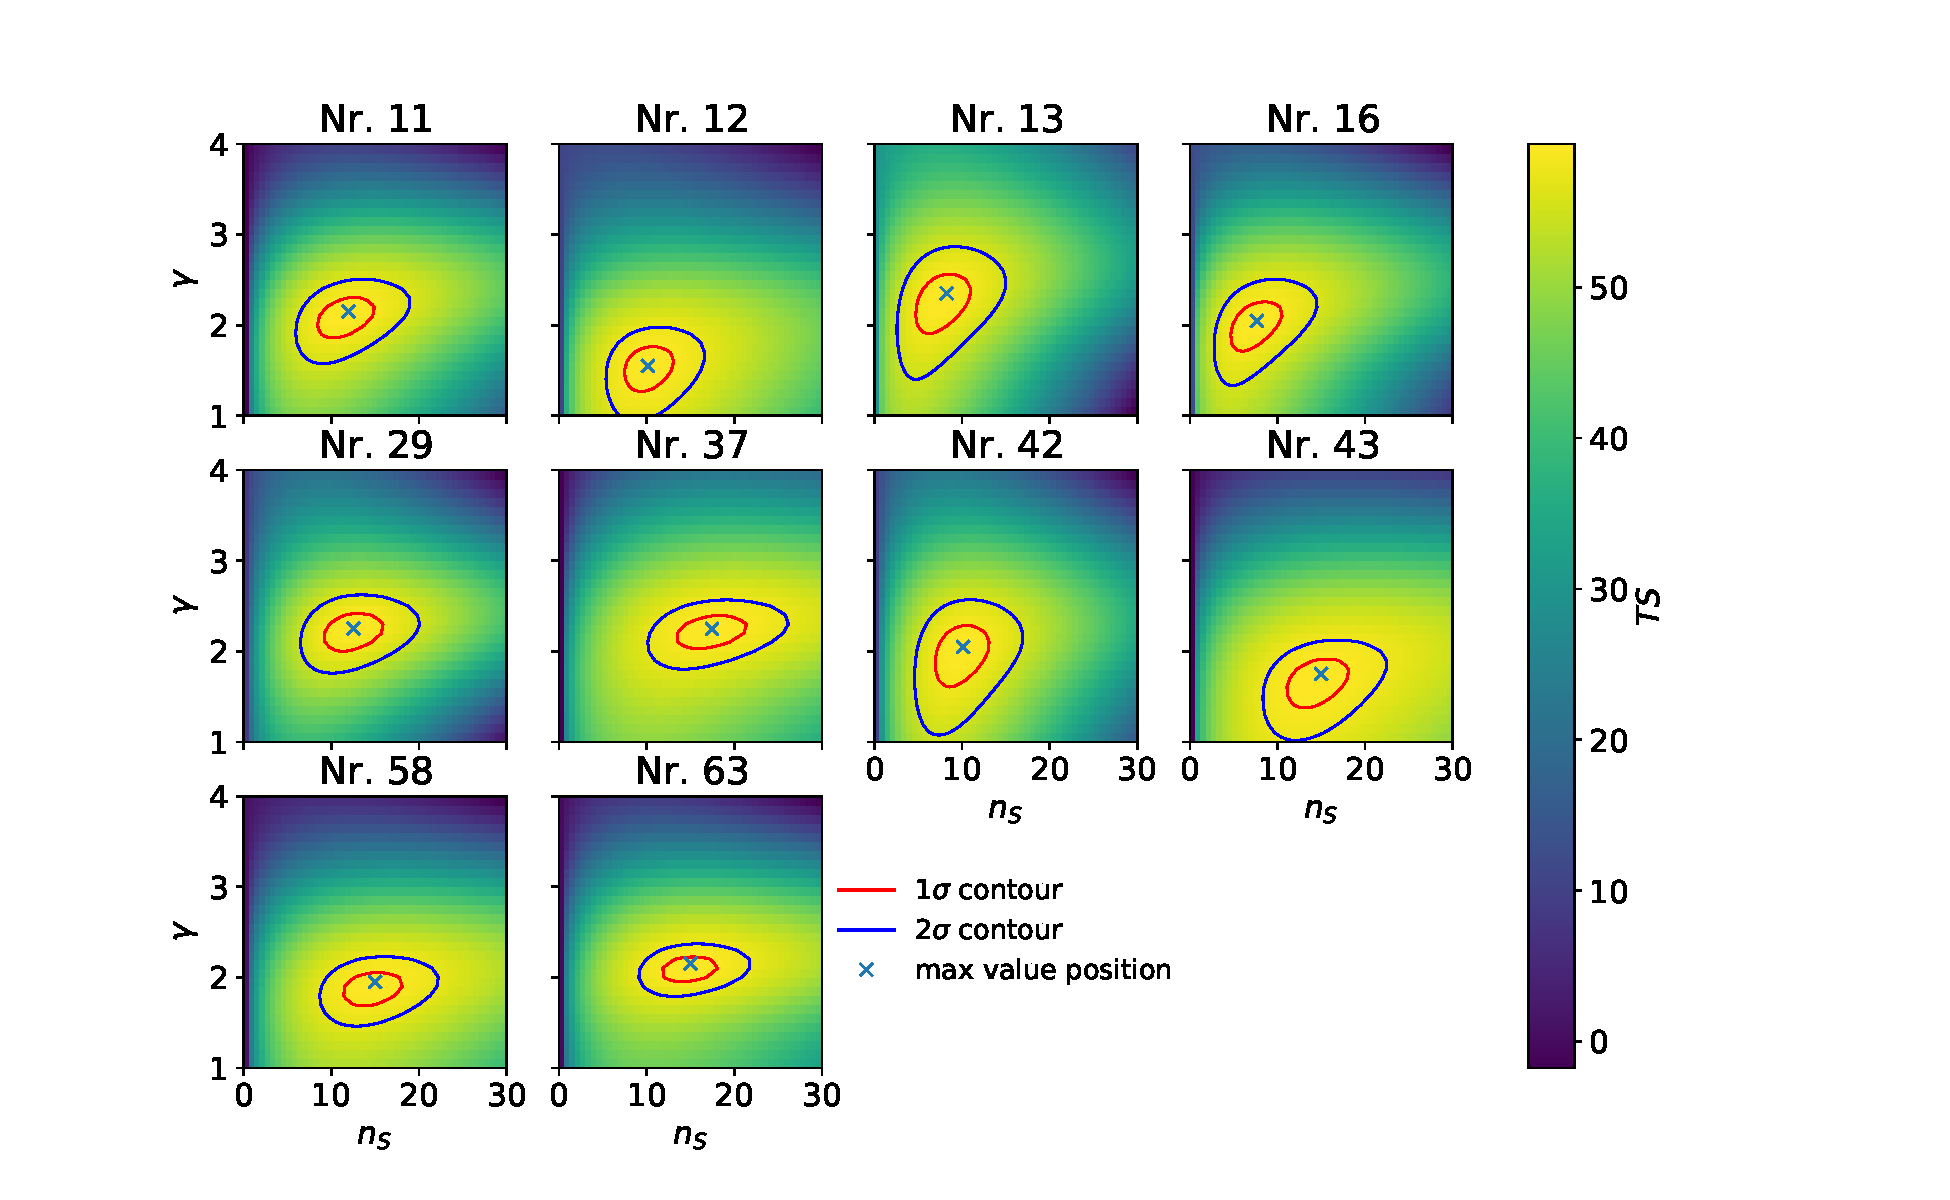
\includegraphics[width=\linewidth]{Plots/appendix/llh_scan.pdf}
    \caption{Scan of the likelihood space for all $\num{10}$ sources with a time window of $\SI{200}{\day}$ for the time-dependent analysis. The scan is in the spectral index $\gamma$ and the signal parameter $n_\text{S}$. The number of induced signal events is $n_S = \num{10}$ with a spectral index of $\gamma = 2$. The maximum test statistic value is marked in the plot including the contours of $\num{1}\sigma$ and $\num{2}\sigma$ and the source number corresponds to the tables \ref{tab:sources_v2} and \ref{tab:sources_v2_2} in the appendix.}
    \label{fig:llh_scan_time_dep_all}
\end{figure}

\begin{figure}
    \centering
    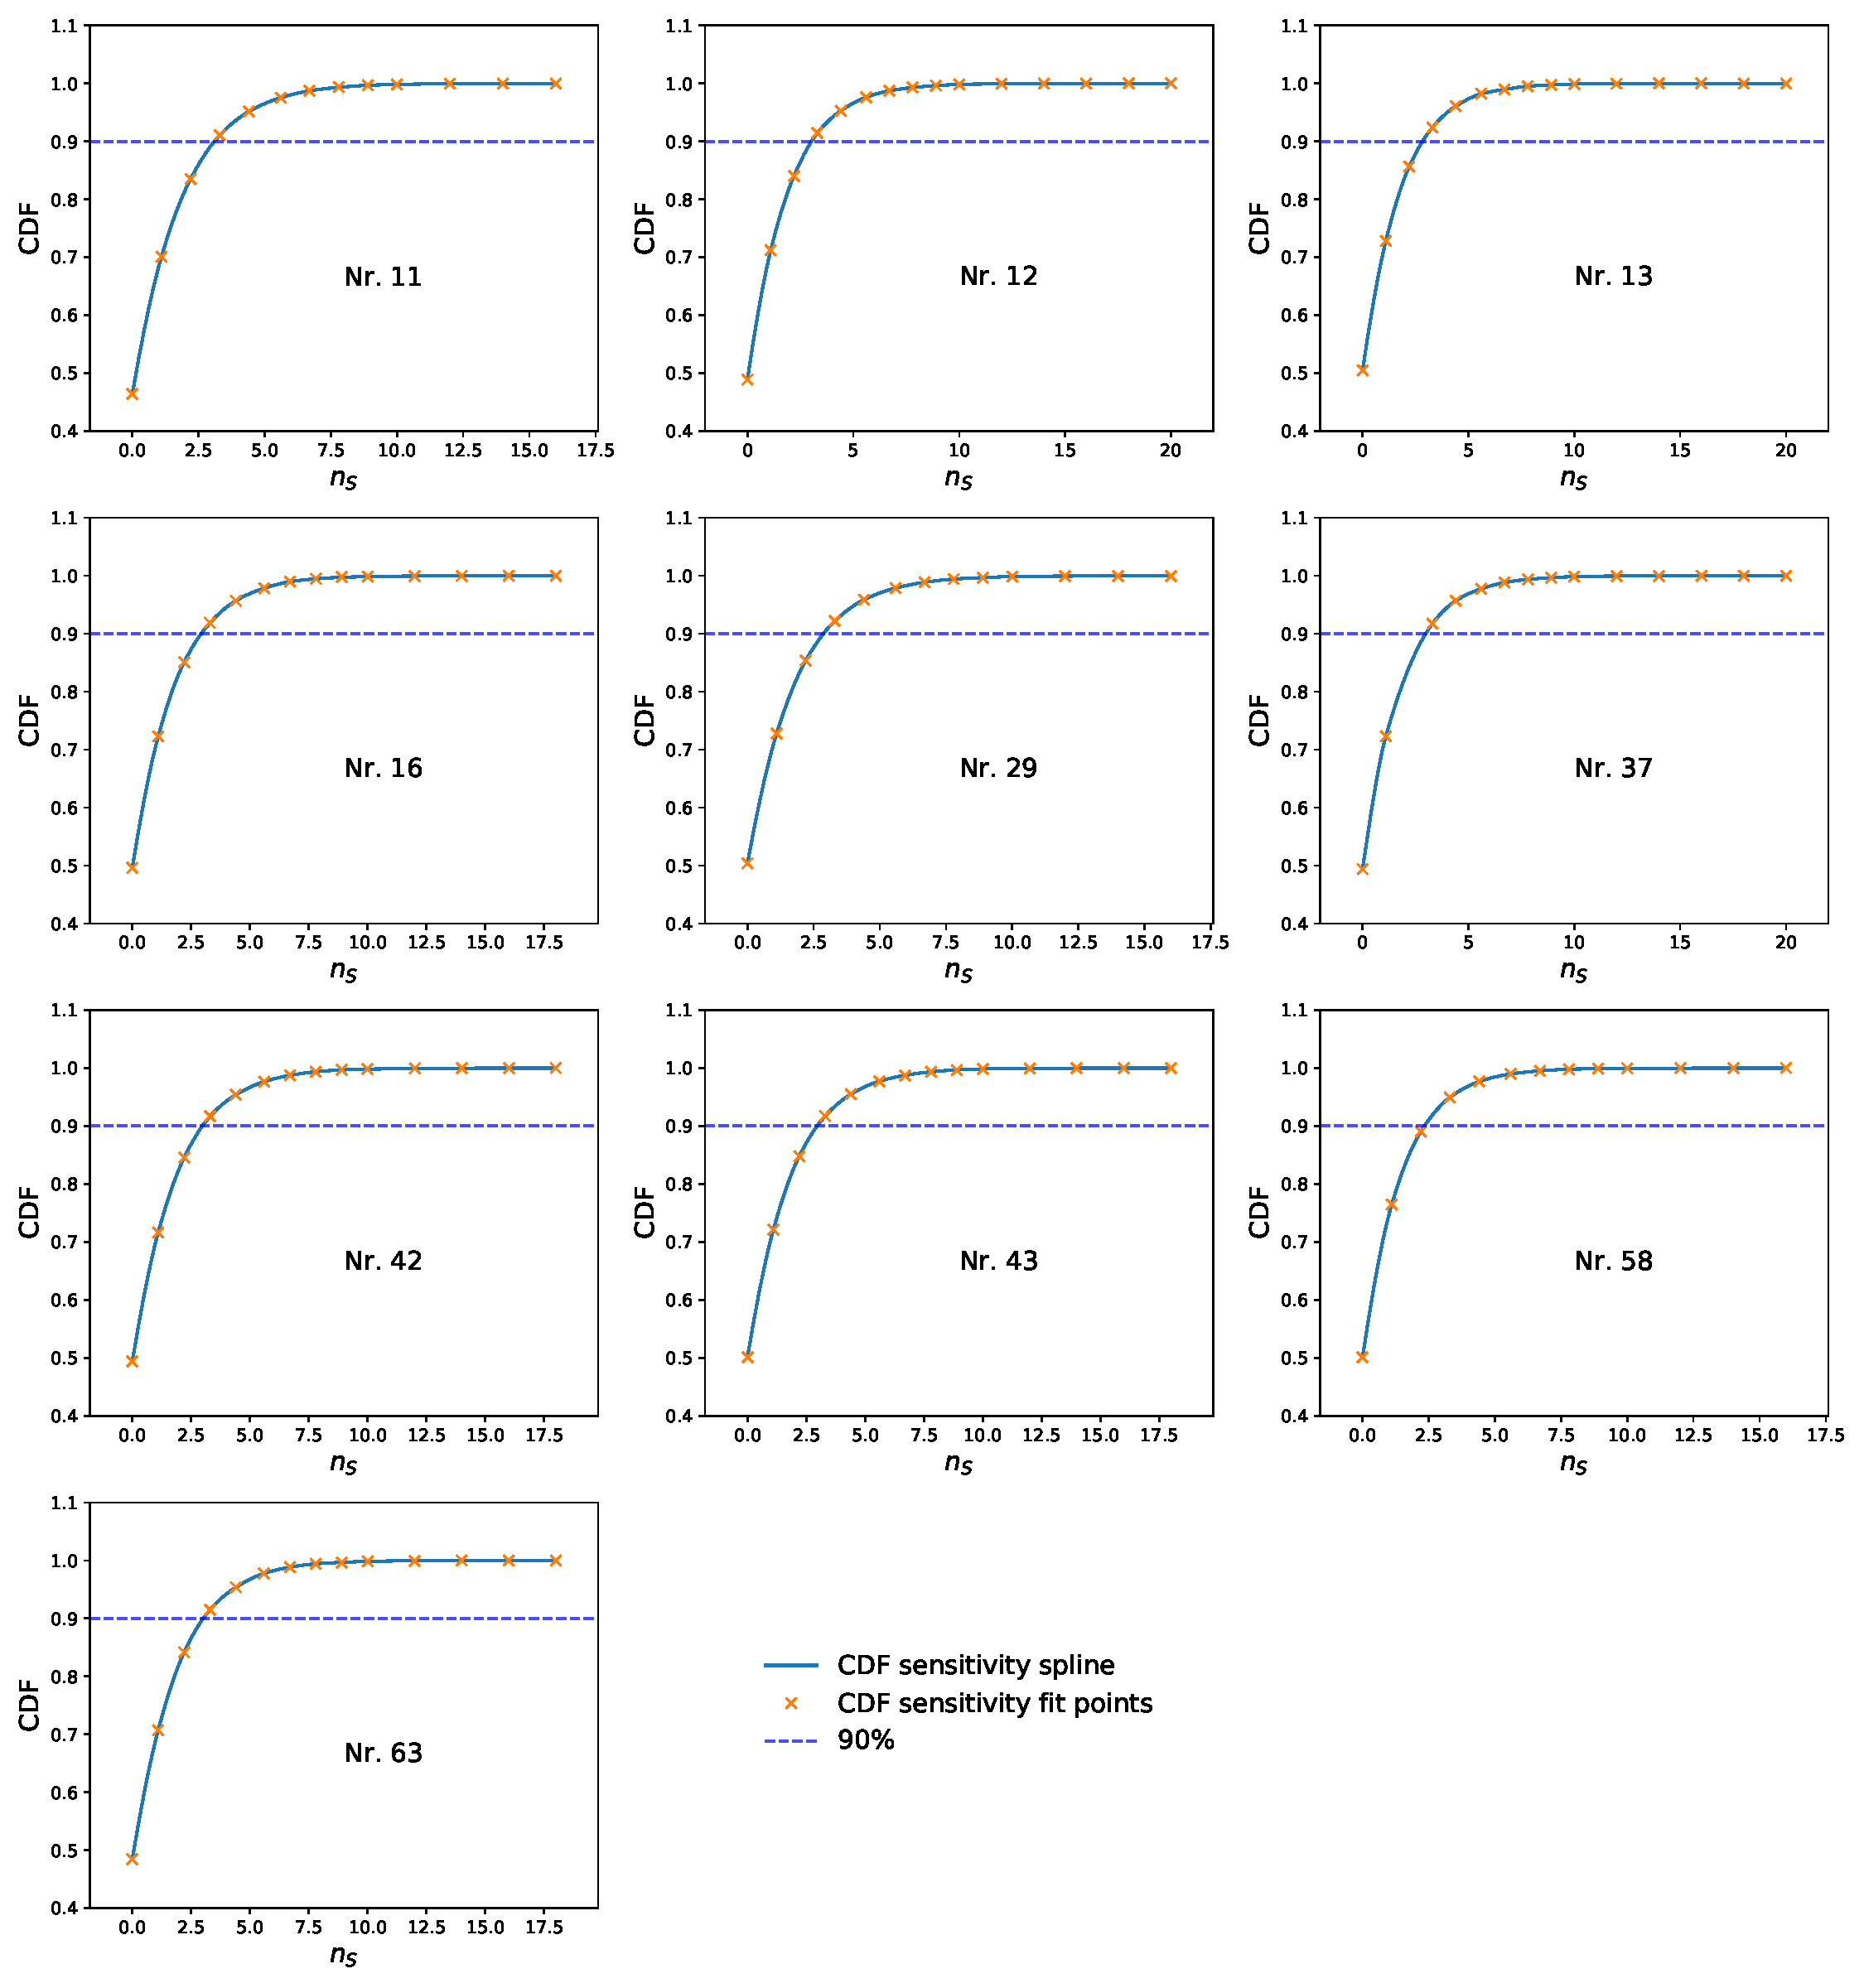
\includegraphics[width=\linewidth]{Plots/appendix/9_years_gfu_gold_time_dep_cdf_sens.pdf}
    \caption{Quantiles of the signal trials for the calculation of the discovery potential for the time-dependent analysis of all $\num{10}$ sources at a spectral index of $\gamma=\num{2}$. A $\chi^2$ CDF fit provides a more accurate estimate of the sought signal parameter $n_\text{S}$ which satisfies the condition of the sensitivity at $\SI{90}{\percent}$ represented via a dashed line.}
    \label{fig:time_dep_cdf_sens}
\end{figure}

\begin{figure}
    \centering
    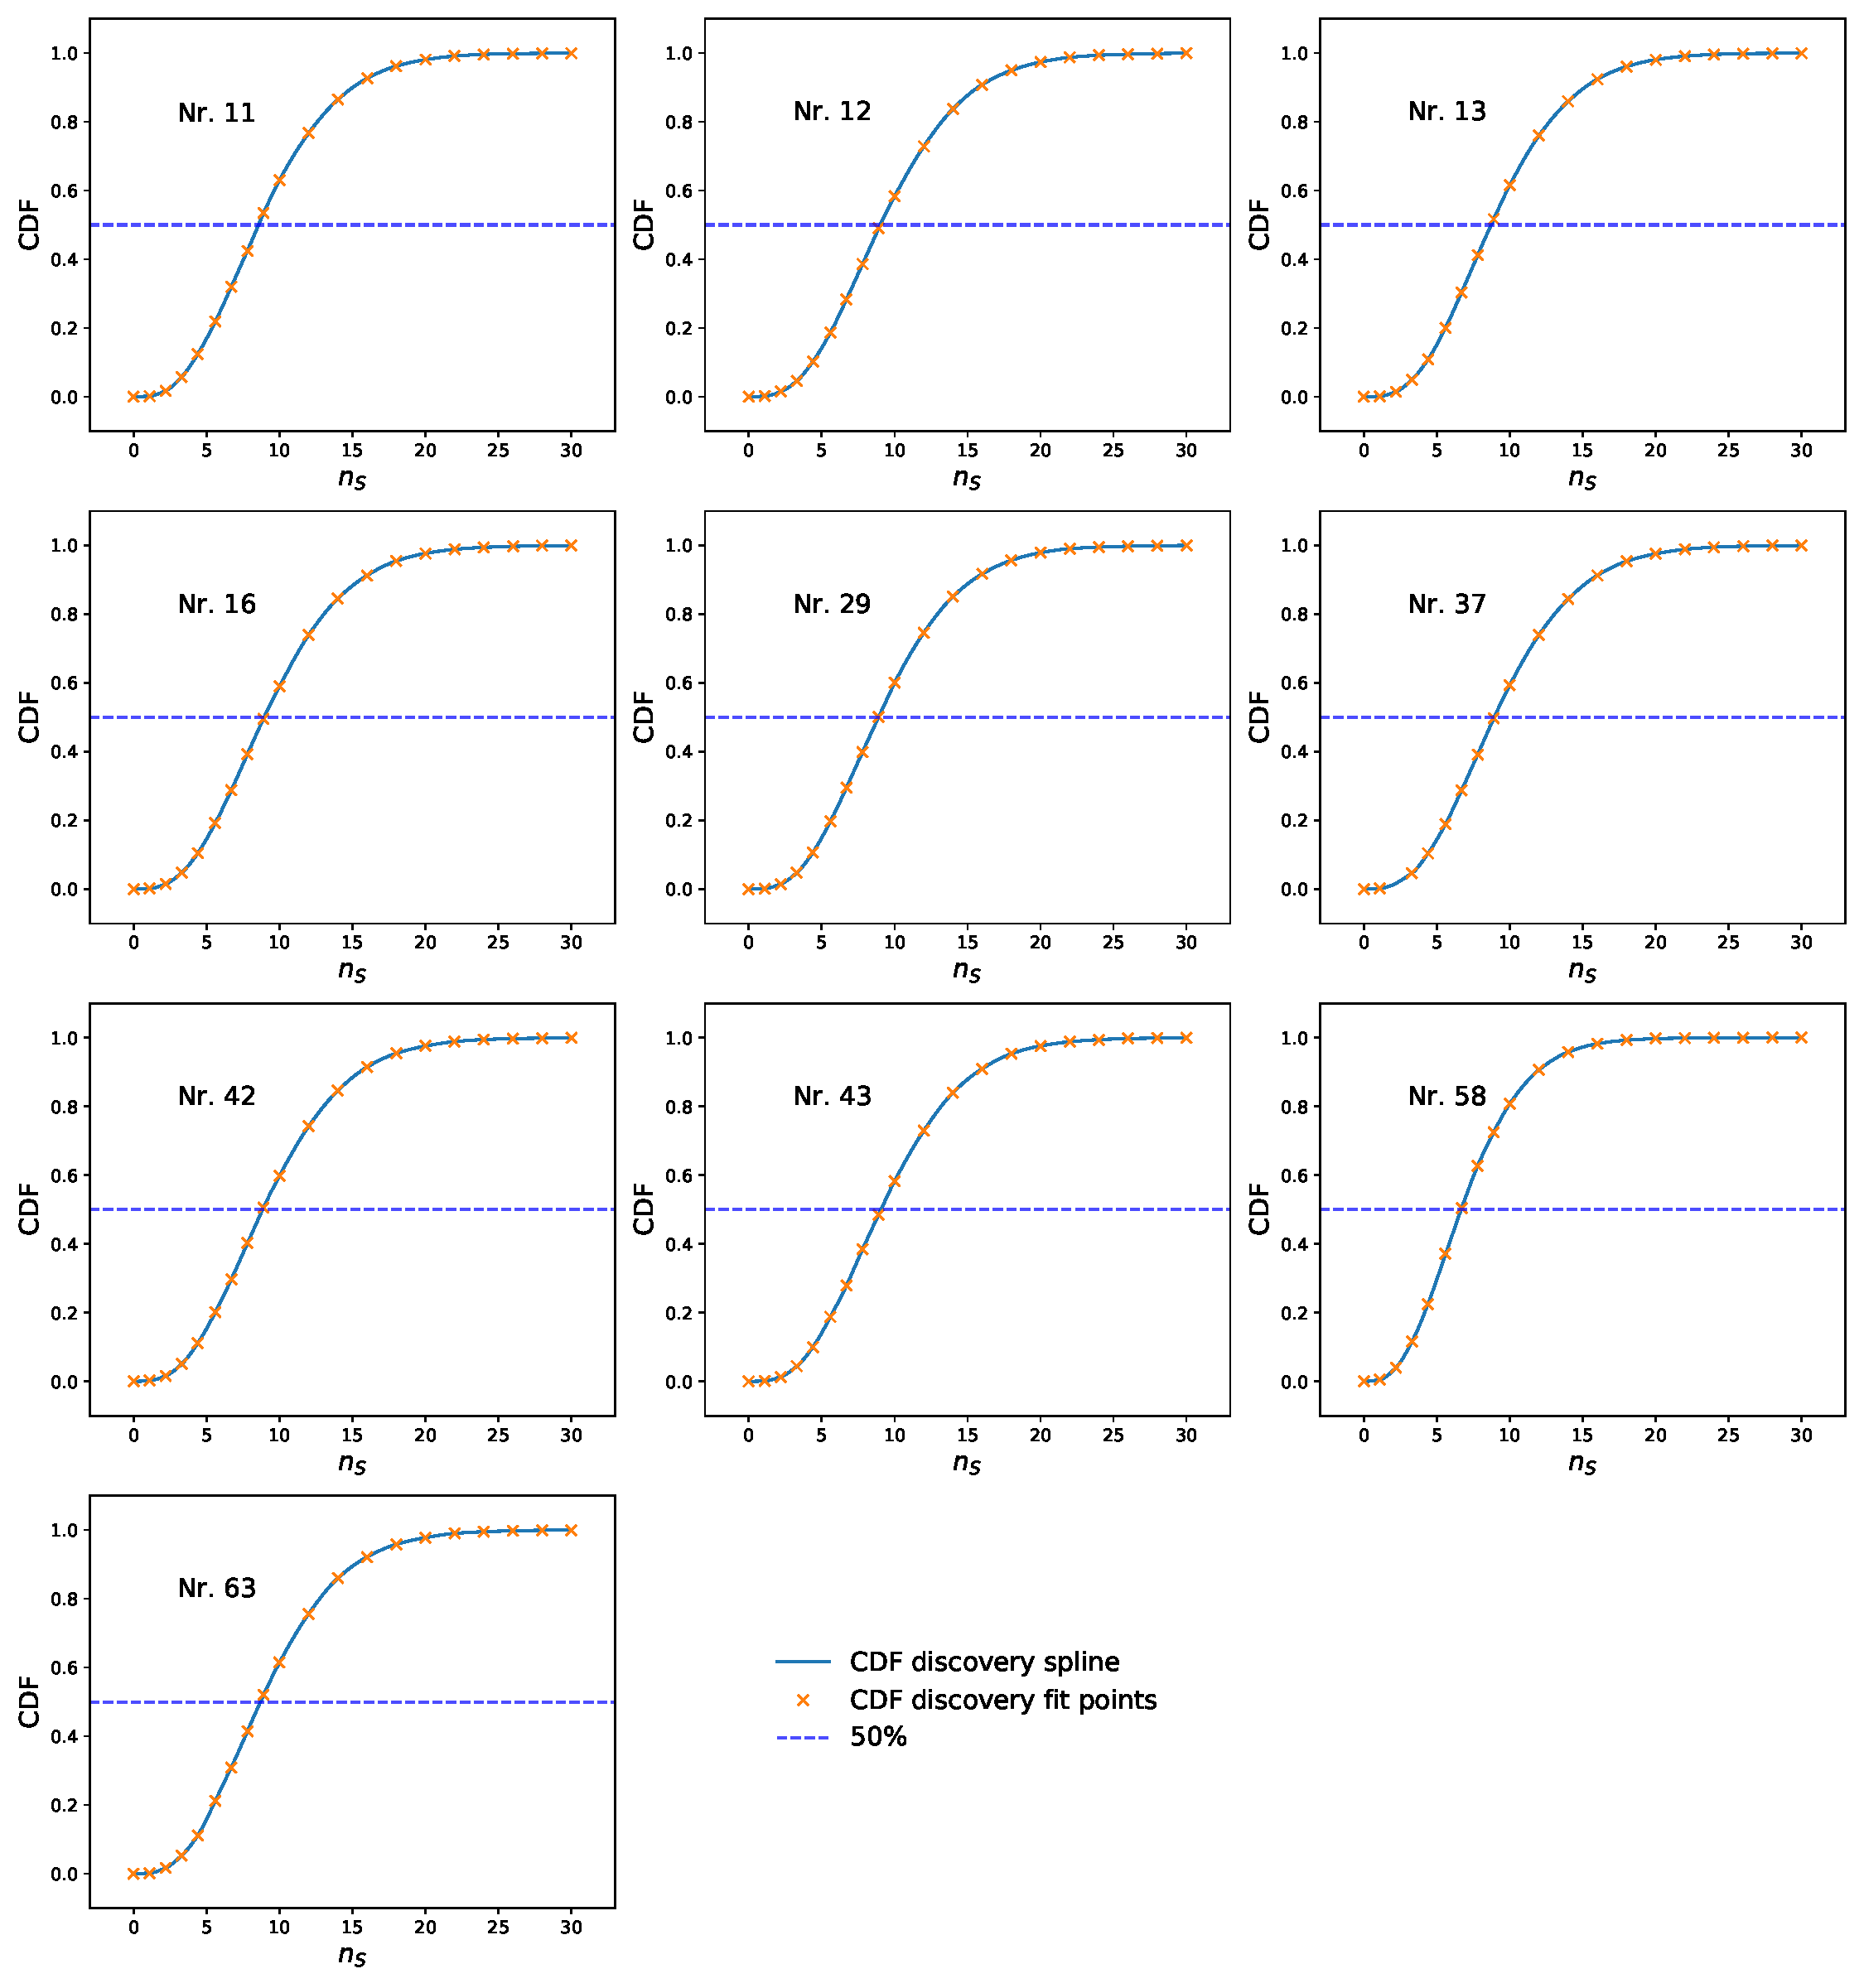
\includegraphics[width=\linewidth]{Plots/appendix/9_years_gfu_gold_time_dep_cdf_disc.pdf}
    \caption{Quantiles of the signal trials for the calculation of the discovery potential for the time-dependent analysis of all $\num{10}$ sources at a spectral index of $\gamma=\num{2}$. A $\chi^2$ CDF fit provides a more accurate estimate of the sought signal parameter $n_\text{S}$ which satisfies the condition of the discovery potential at $\SI{50}{\percent}$ represented via a dashed line.}
    \label{fig:time_dep_cdf_disc}
\end{figure}

\begin{figure}
    \centering
    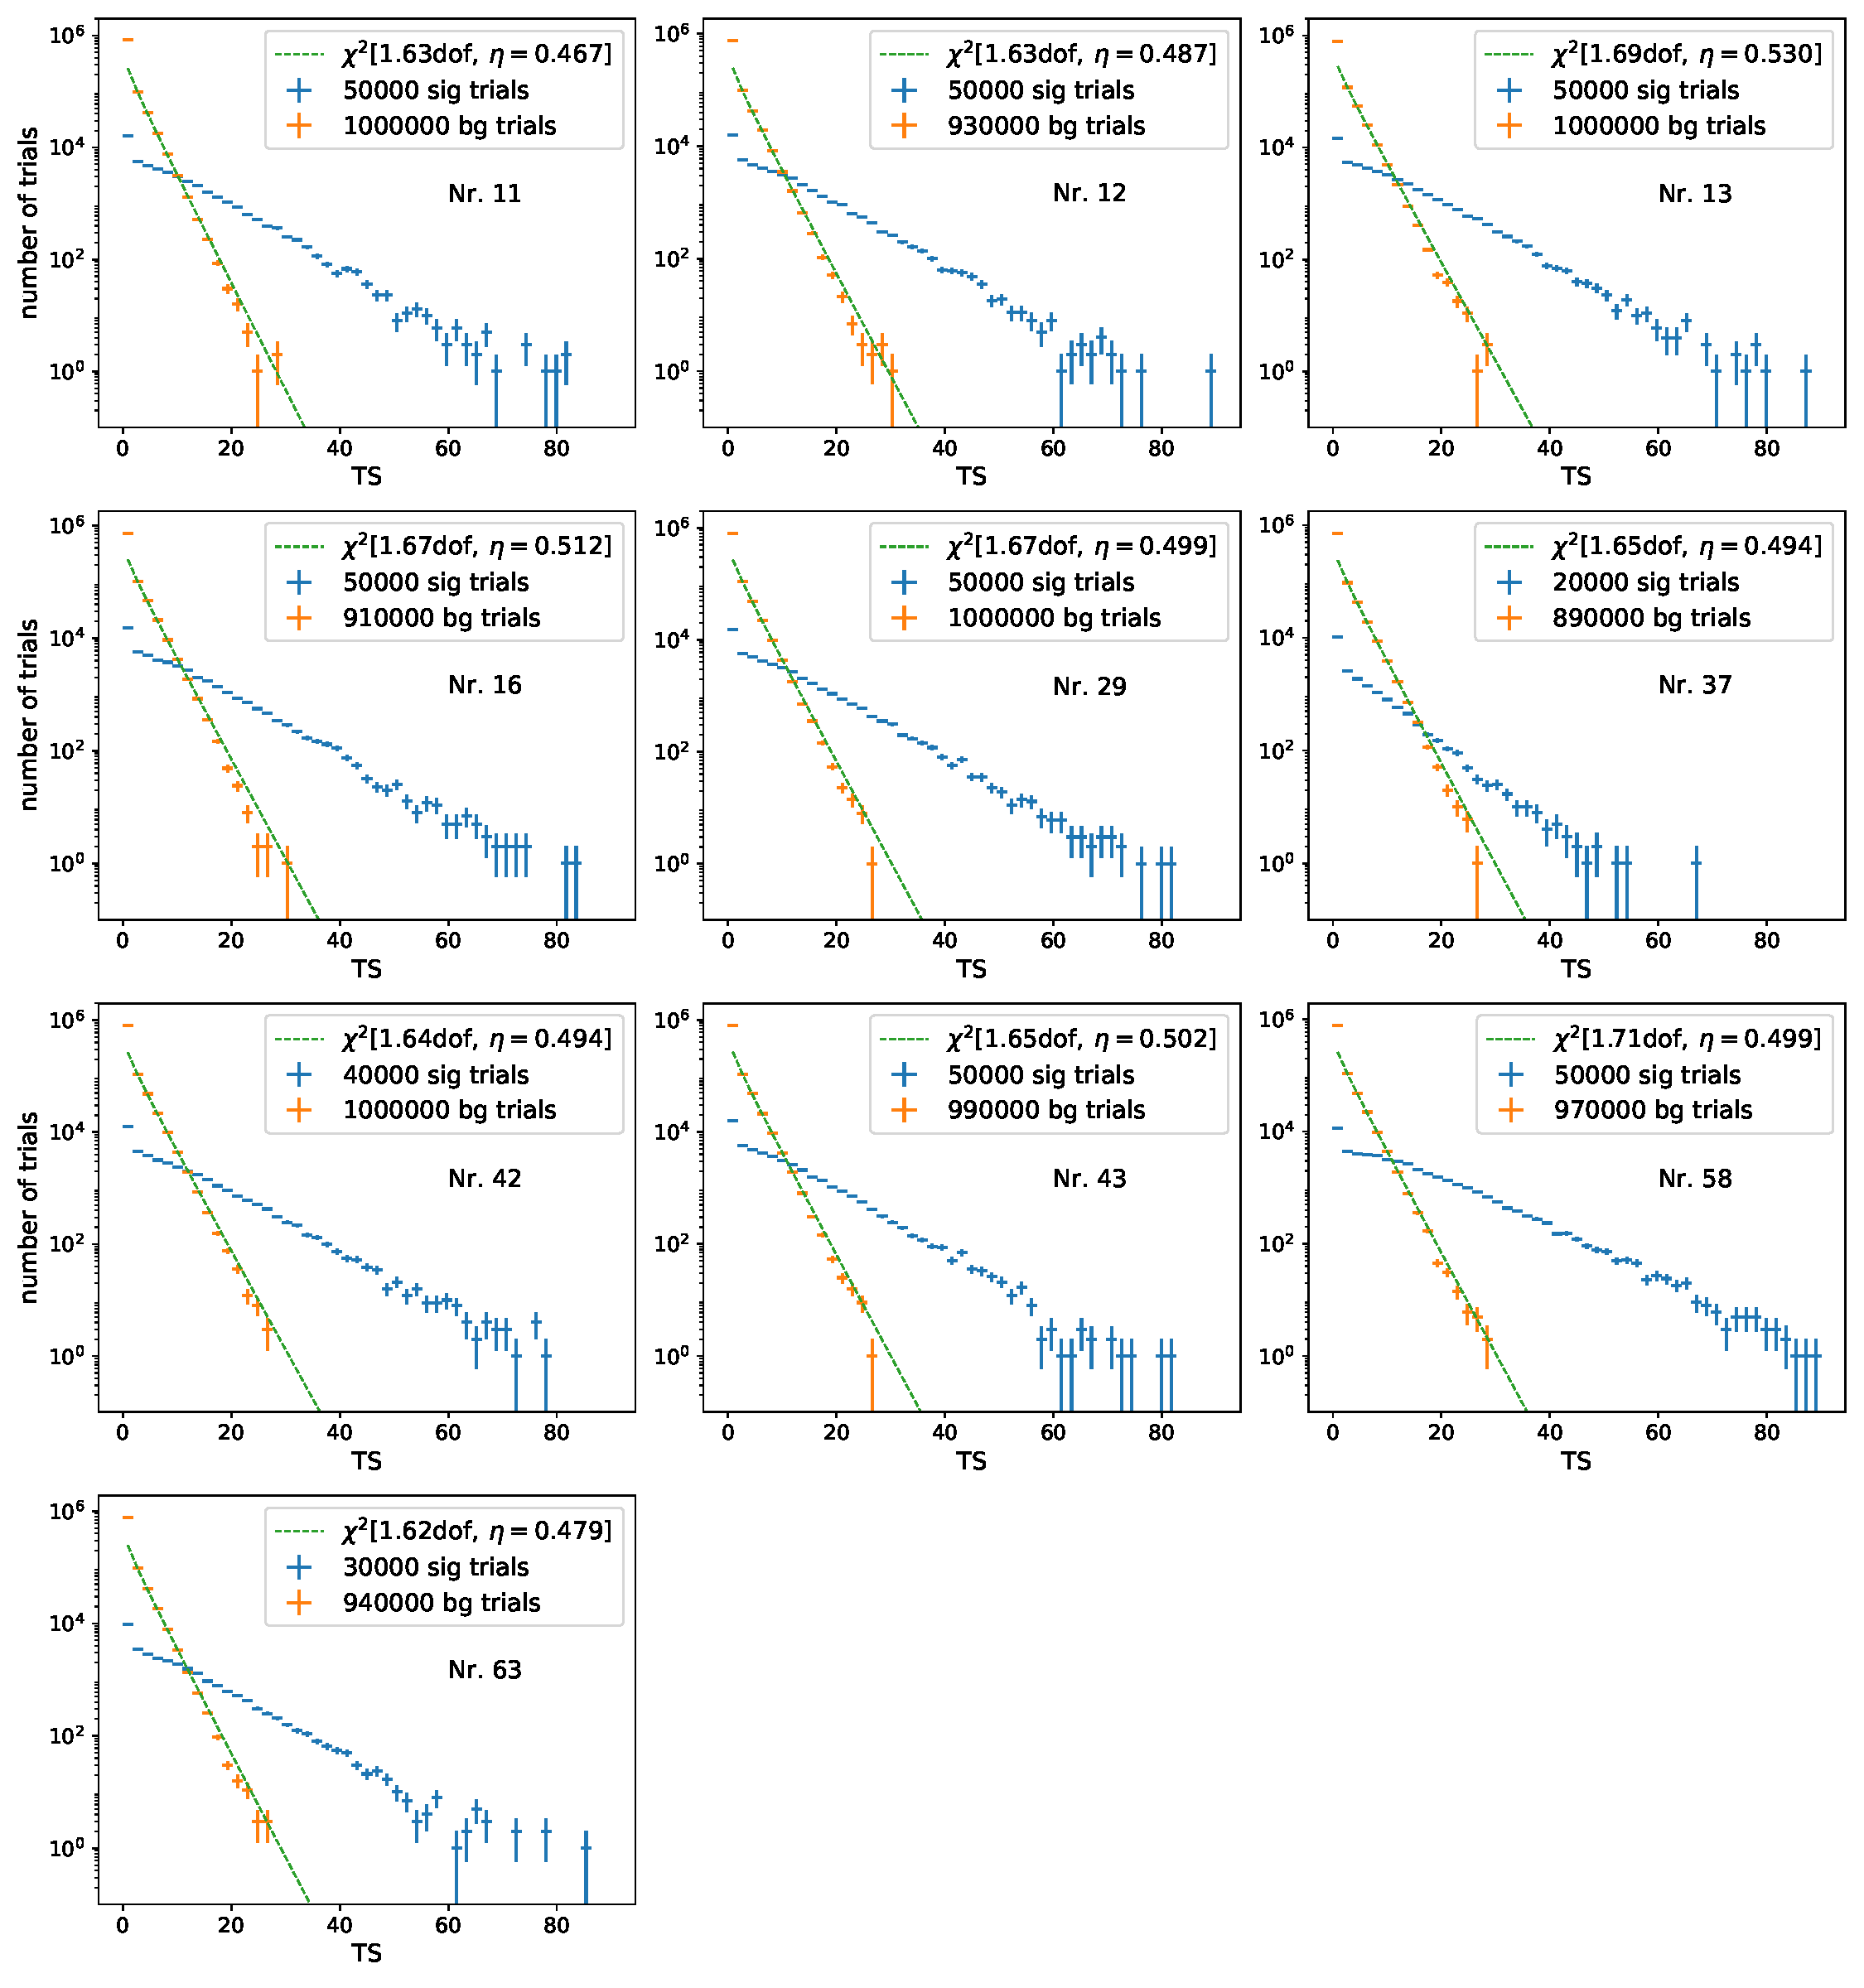
\includegraphics[width=\linewidth]{Plots/appendix/9_years_gfu_gold_time_dep_sig_sens_ts.pdf}
    \caption{Histogram of the background trials for the time-dependent analysis for all $\num{10}$ sources. Shown is also the set of signal trials with the number of injected signal events closest to satisfying the condition to calculate the sensitivity. The median of the background test statistics is not plotted as it is very close to the origin for all sources.}
    \label{fig:time_dep_sig_sens_ts}
\end{figure}

\begin{figure}
    \centering
    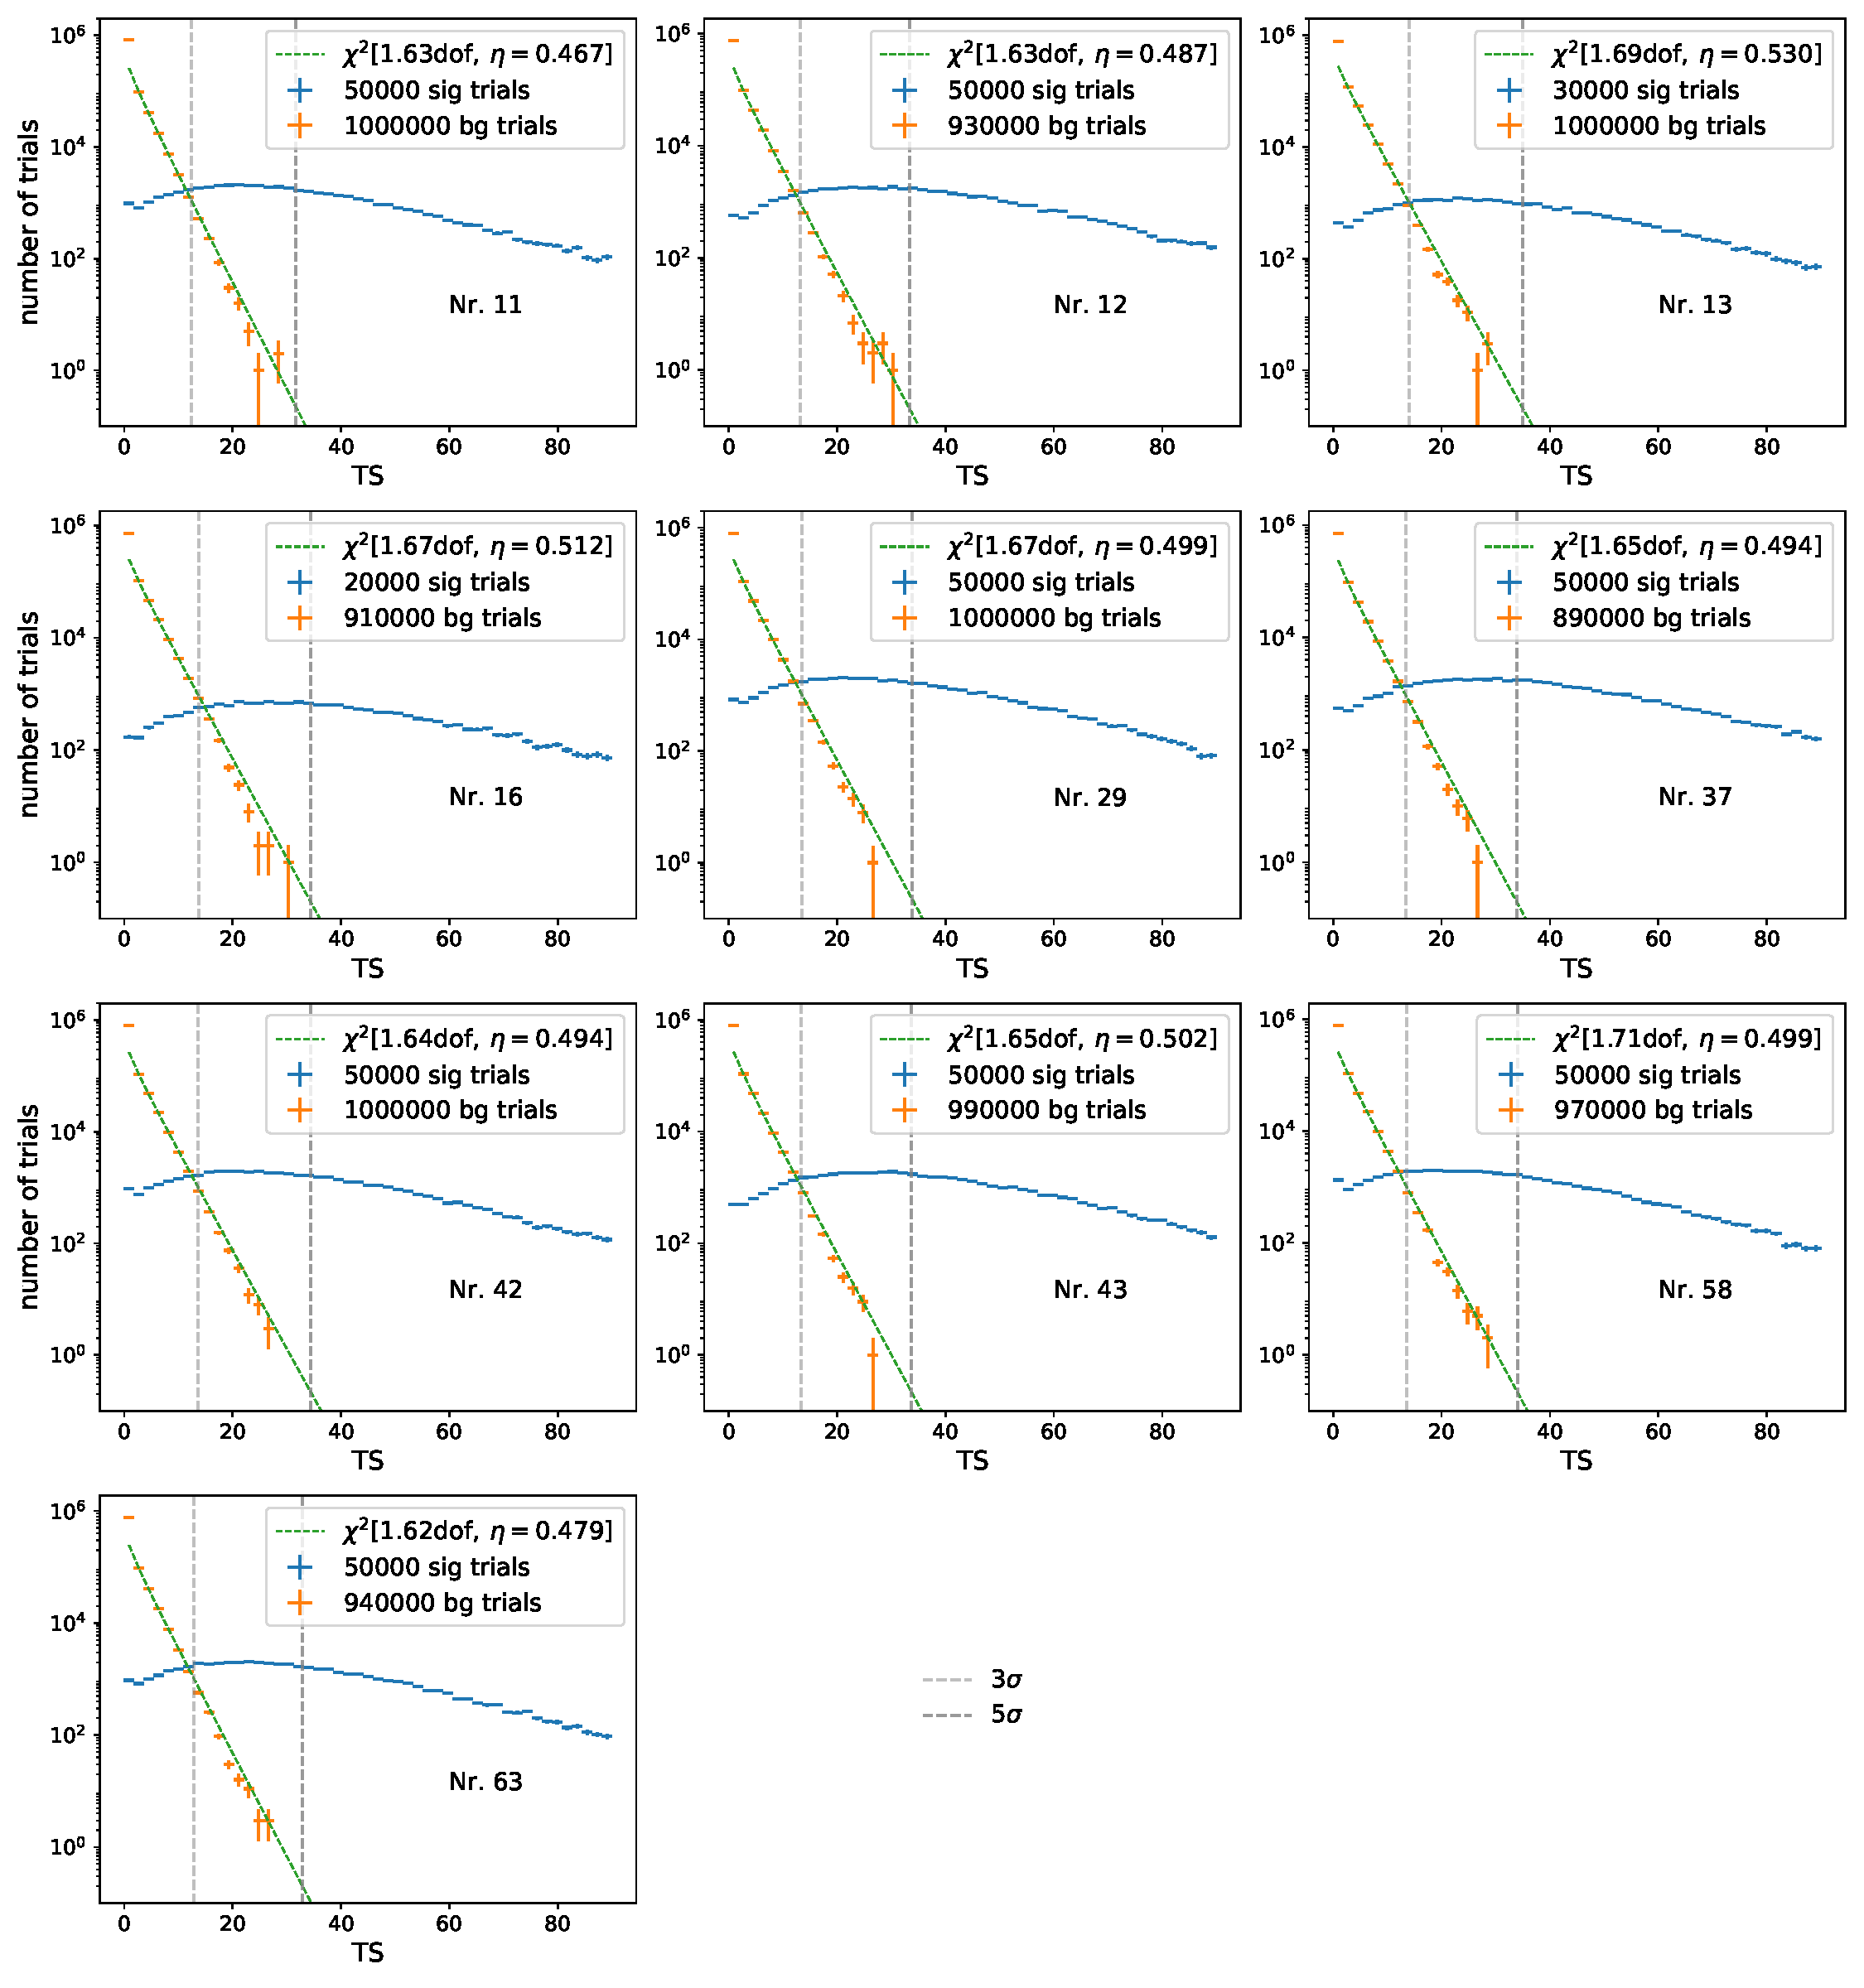
\includegraphics[width=\linewidth]{Plots/appendix/9_years_gfu_gold_time_dep_sig_disc_ts.pdf}
    \caption{Histogram of the background trials for the time-dependent analysis for all $\num{10}$ sources. Shown is also the set of signal trials with the number of injected signal events closest to satisfying the condition to calculate the discovery potential. The grey dashed lines represent $\num{3}\sigma$ and $\num{5}\sigma$ of the background test statistic.}
    \label{fig:time_dep_sig_disc_ts}
\end{figure}

\begin{figure}
    \centering
    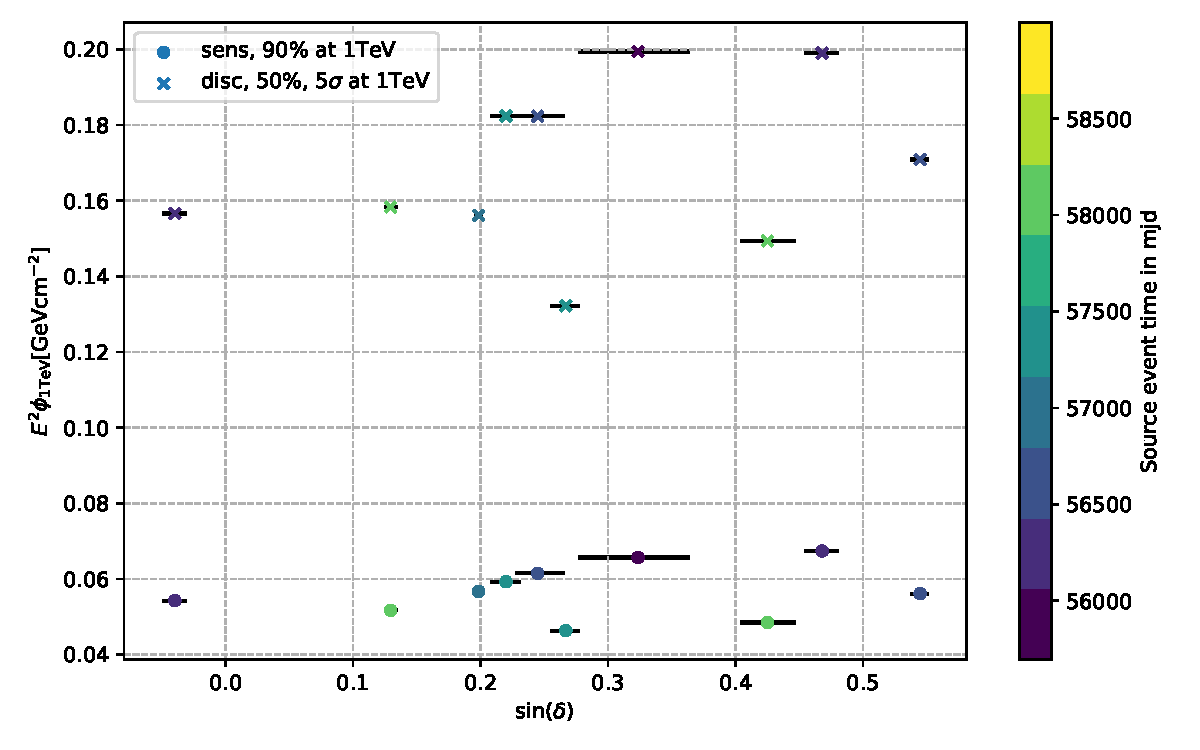
\includegraphics[width=\linewidth]{Plots/appendix/time_dep_sens_disc_dec_time_2.pdf}
    \caption{Sensitivities and discovery potentials for all $\num{10}$ sources in dependence of their position at a reference energy of $E_0 = \SI{100}{\tera\electronvolt}$ for the time-dependent analysis. The colour represents the arrival time of the source event and the errorbars the uncertainty in declination.}
    \label{fig:sens_disc_time_dep_dec}
\end{figure}

\begin{figure}
    \centering
    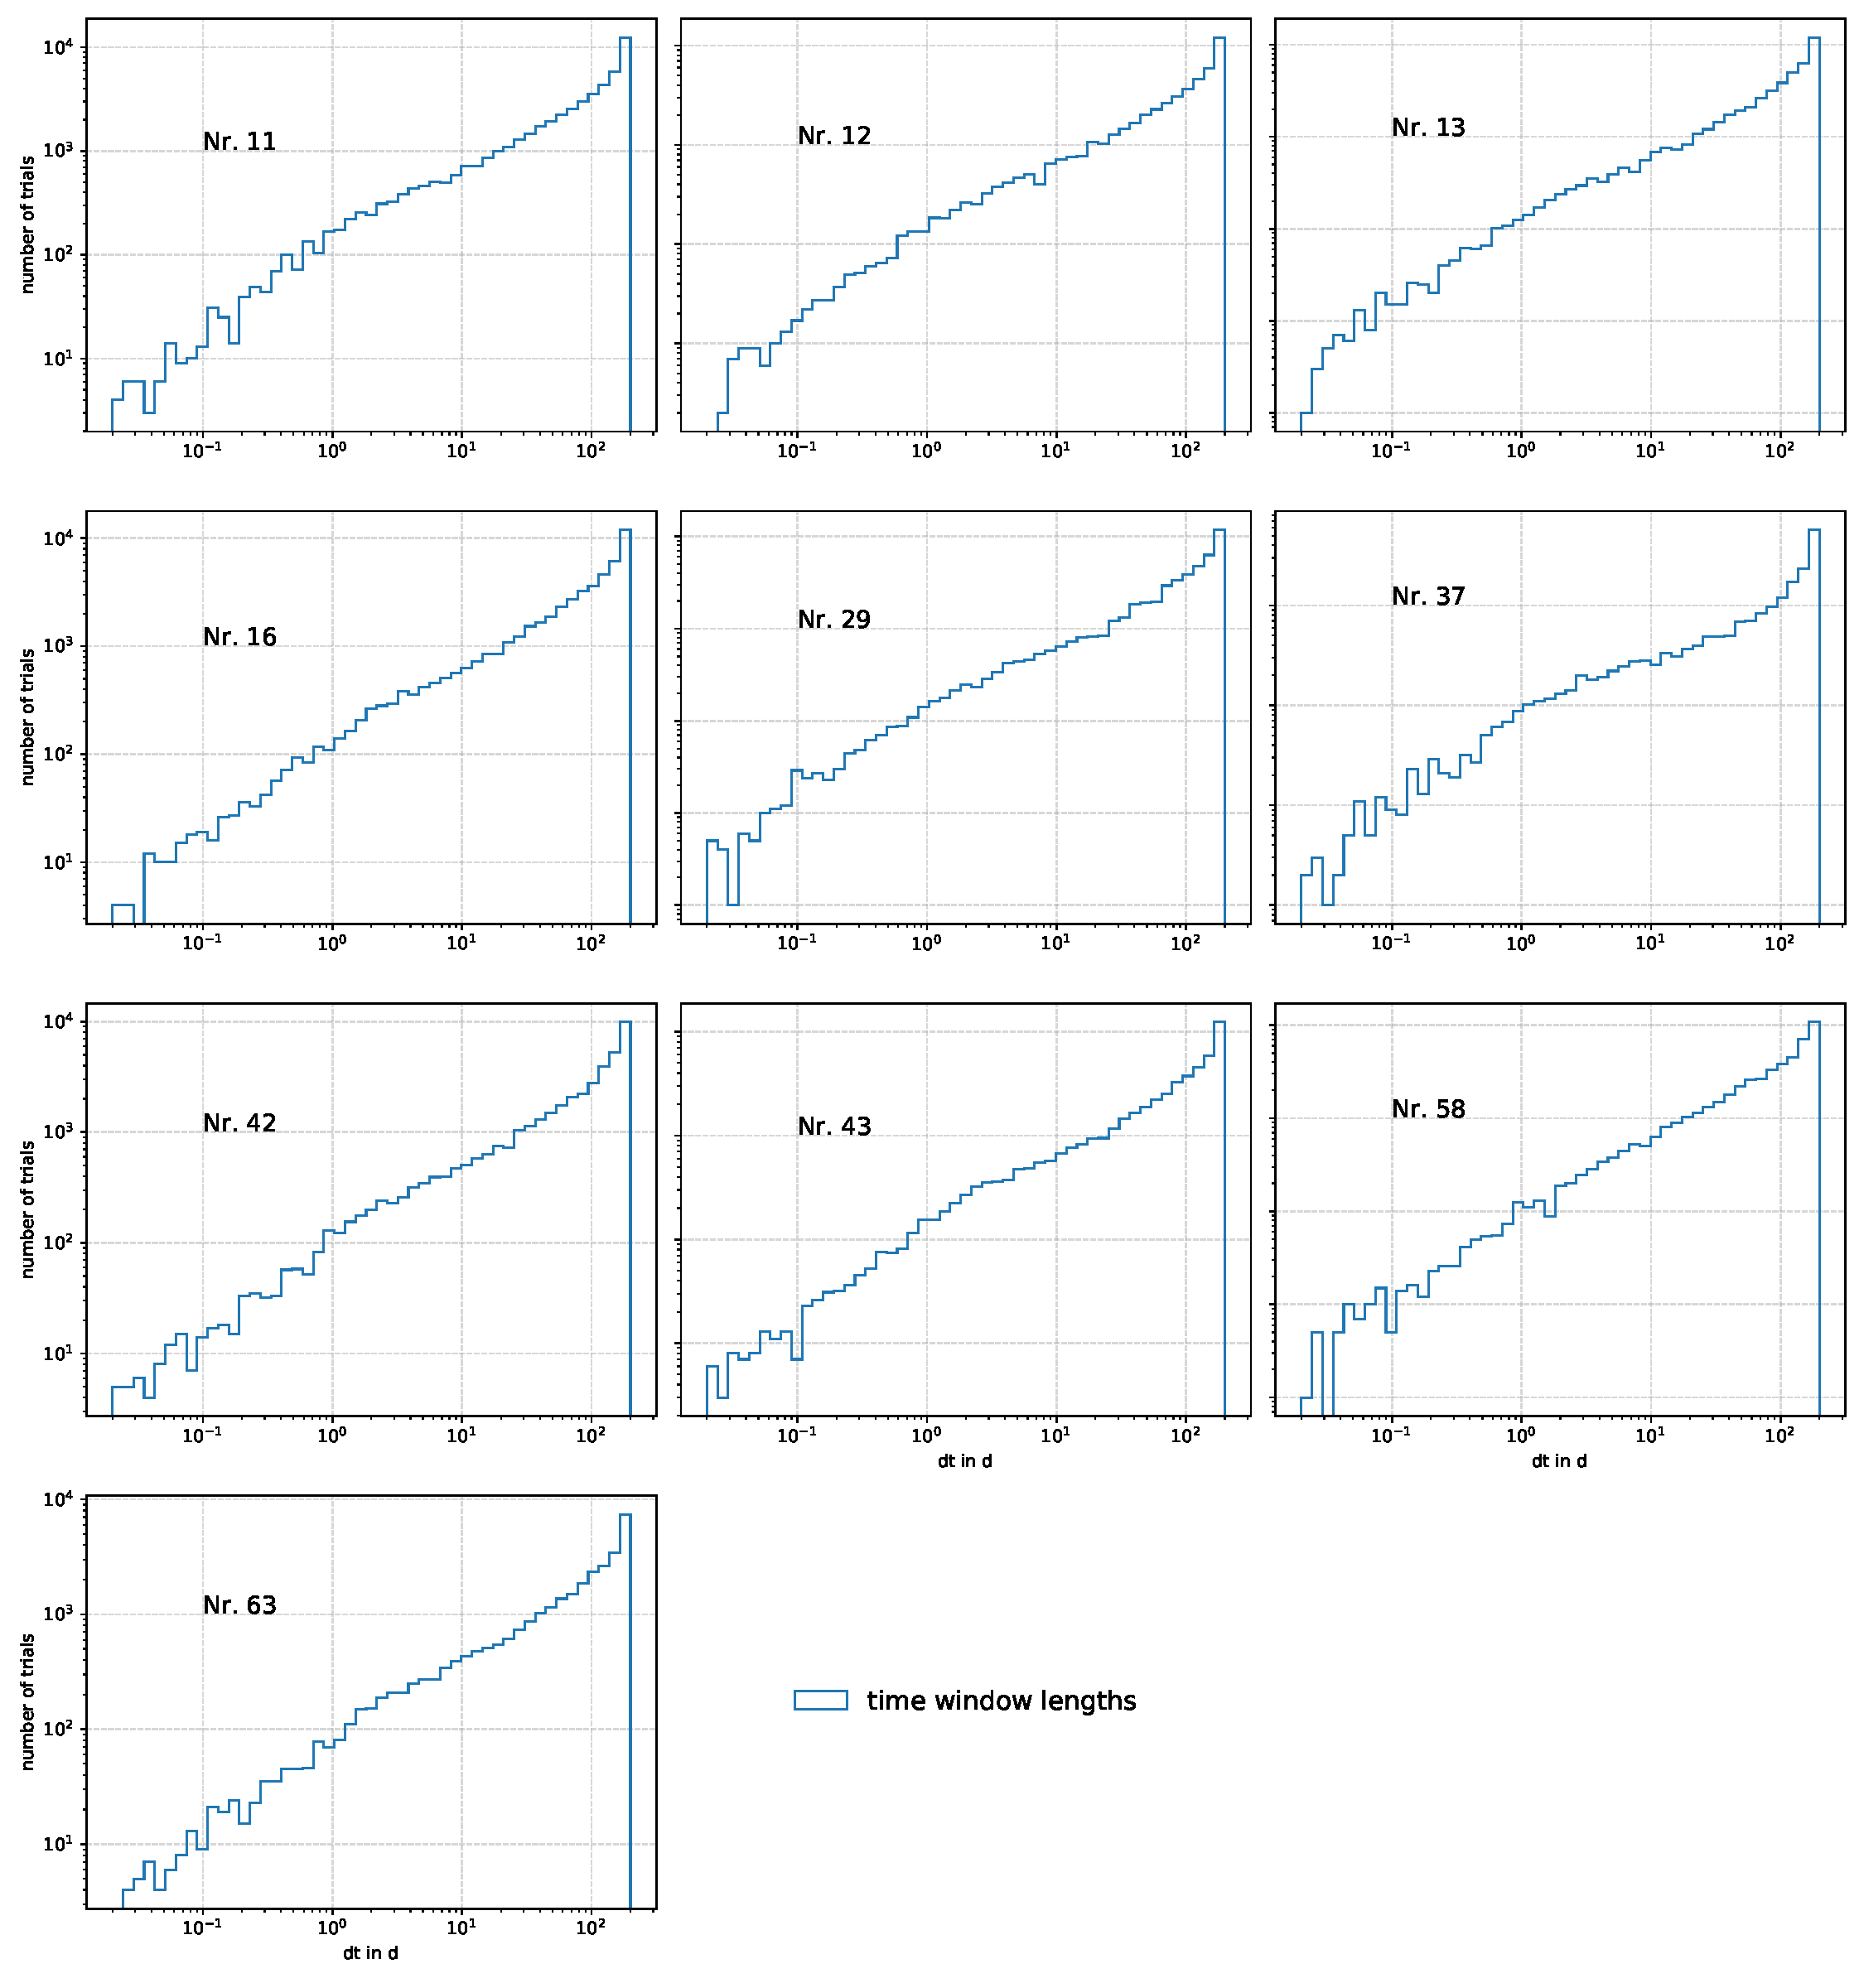
\includegraphics[width=\linewidth]{Plots/appendix/9_years_gfu_gold_time_dep_sens_dt.pdf}
    \caption{Histograms of the time window lengths $dt$ in days of all $\num{10}$ sources for the time-dependent analysis for the set of signal trials with the number of injected signal events closest to satisfying the condition to calculate the sensitivity.}
    \label{fig:sens_dt_all}
\end{figure}

\begin{figure}
    \centering
    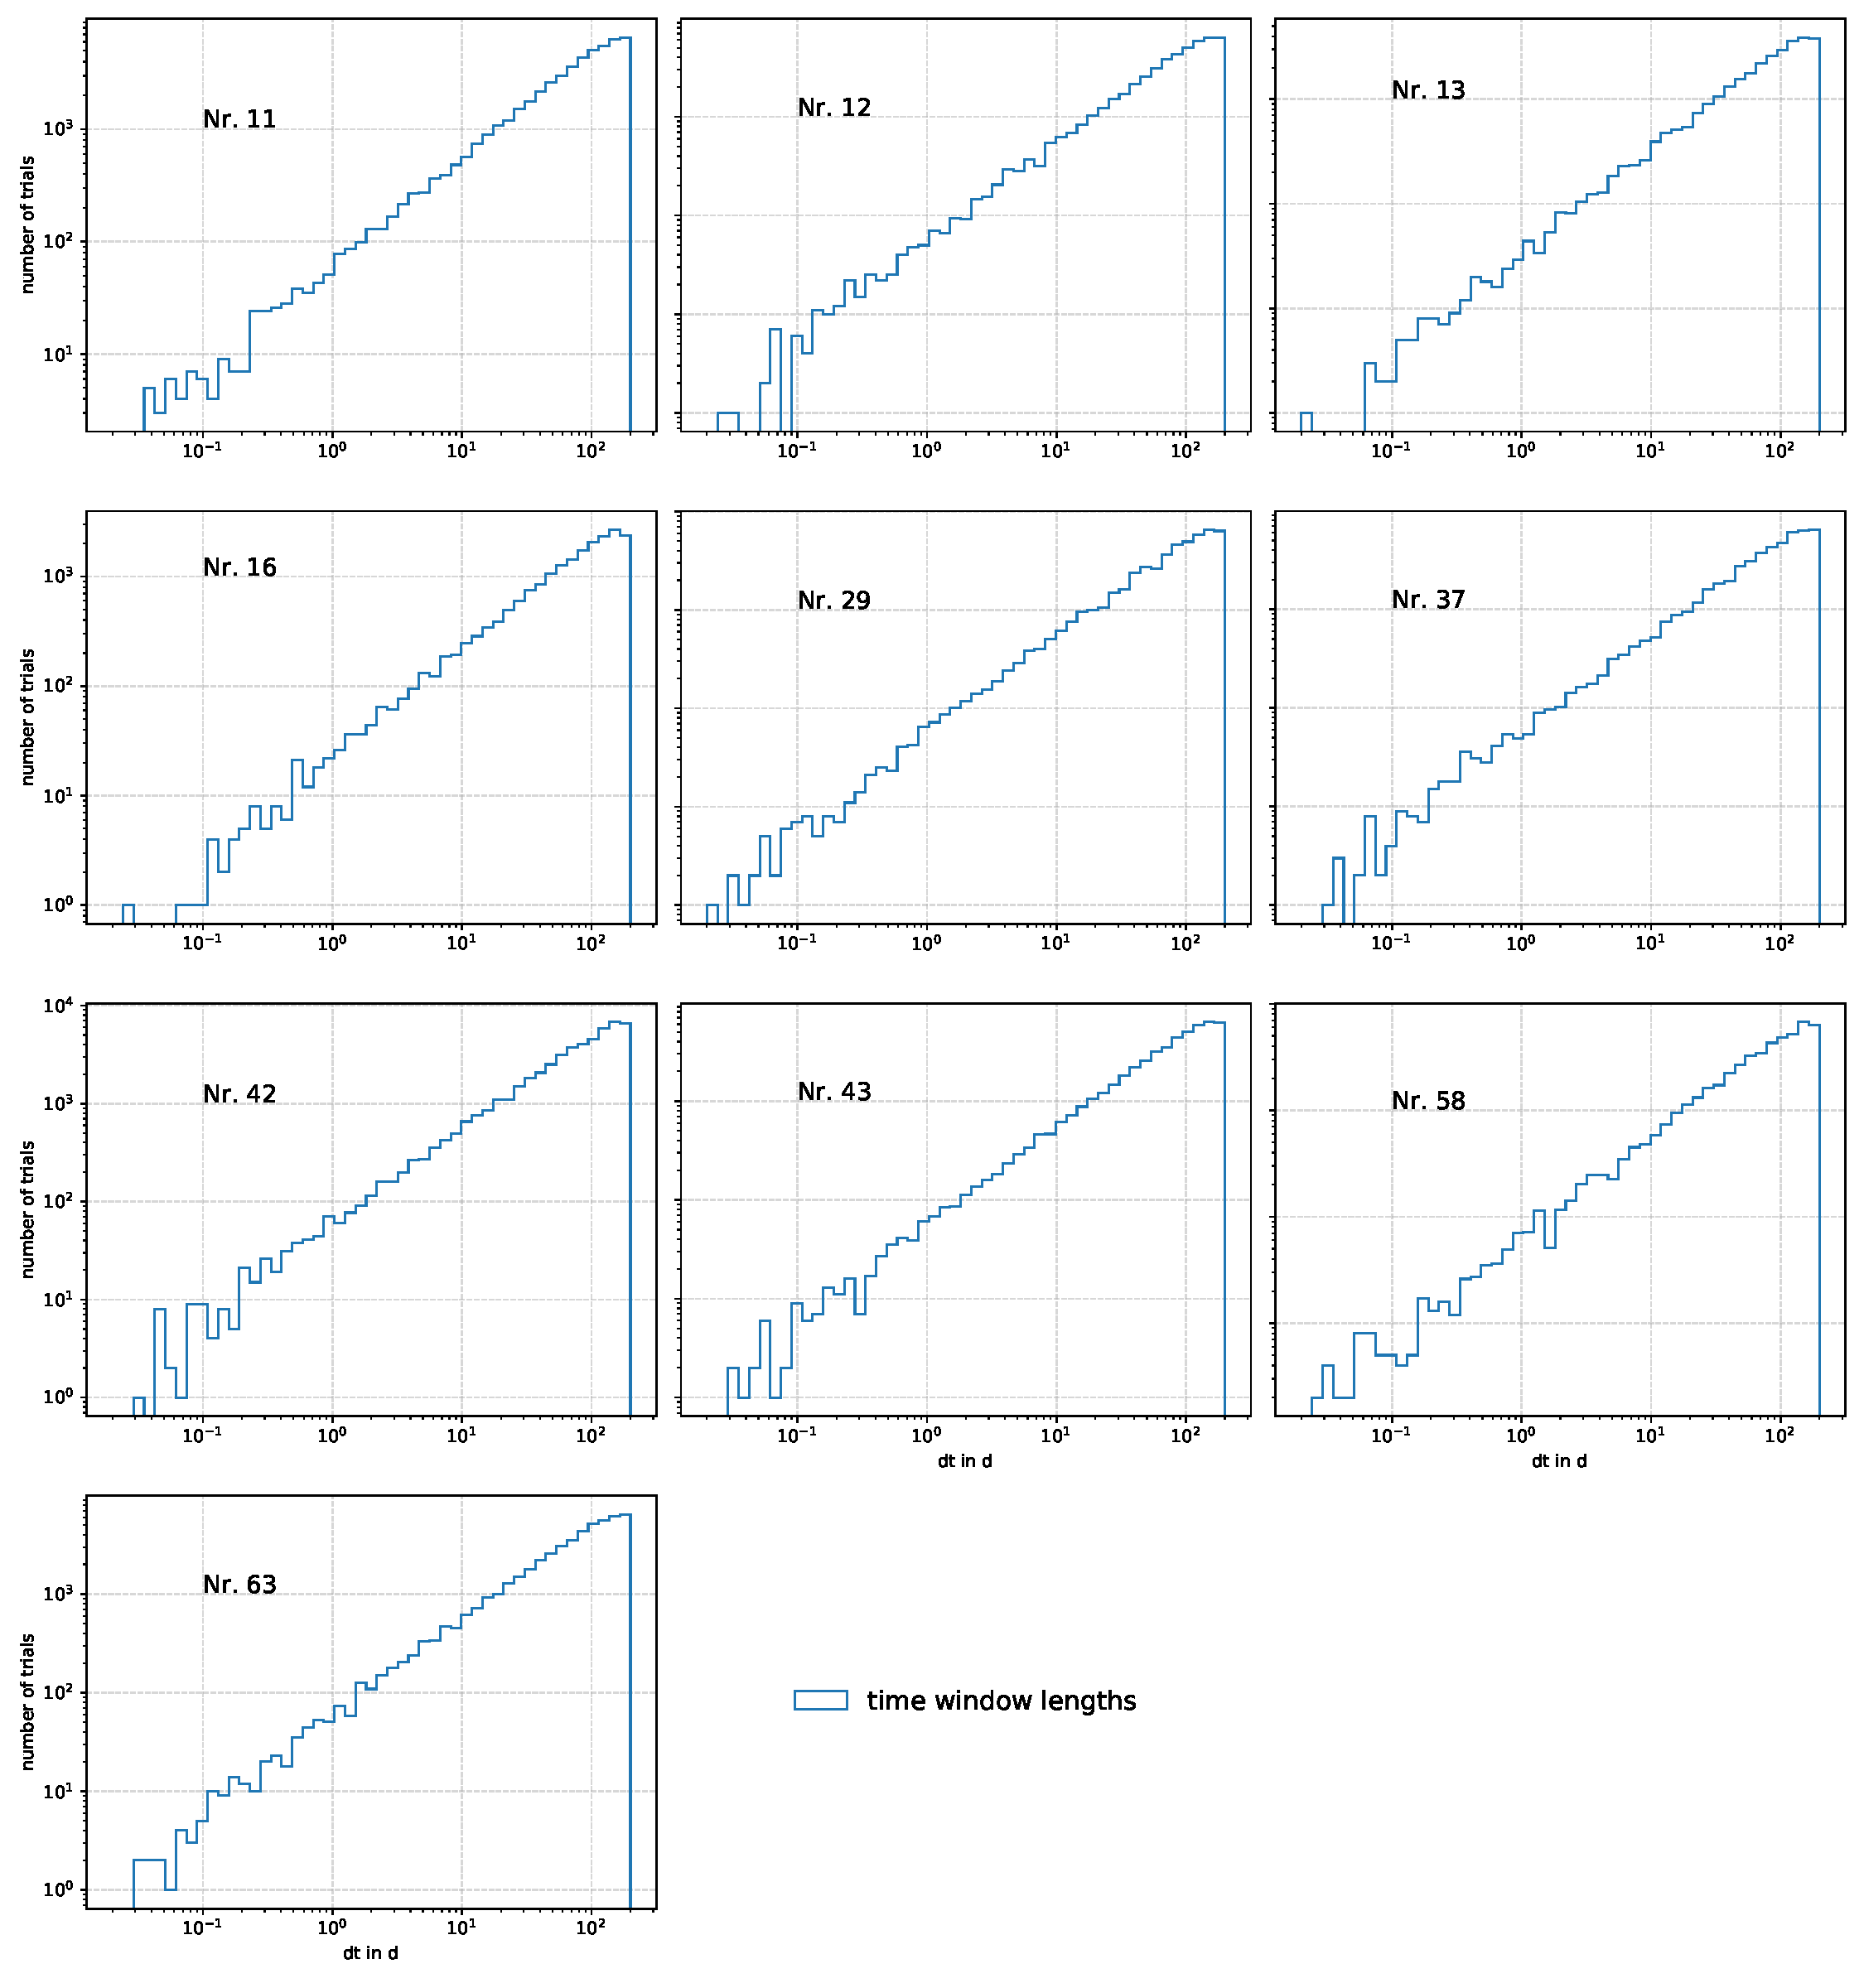
\includegraphics[width=\linewidth]{Plots/appendix/9_years_gfu_gold_time_dep_disc_dt.pdf}
    \caption{Histograms of the time window lengths $dt$ in days of all $\num{10}$ sources for the time-dependent analysis for the set of signal trials with the number of injected signal events closest to satisfying the condition to calculate the discovery potential.}
    \label{fig:disc_dt_all}
\end{figure}

\begin{figure}
    \centering
    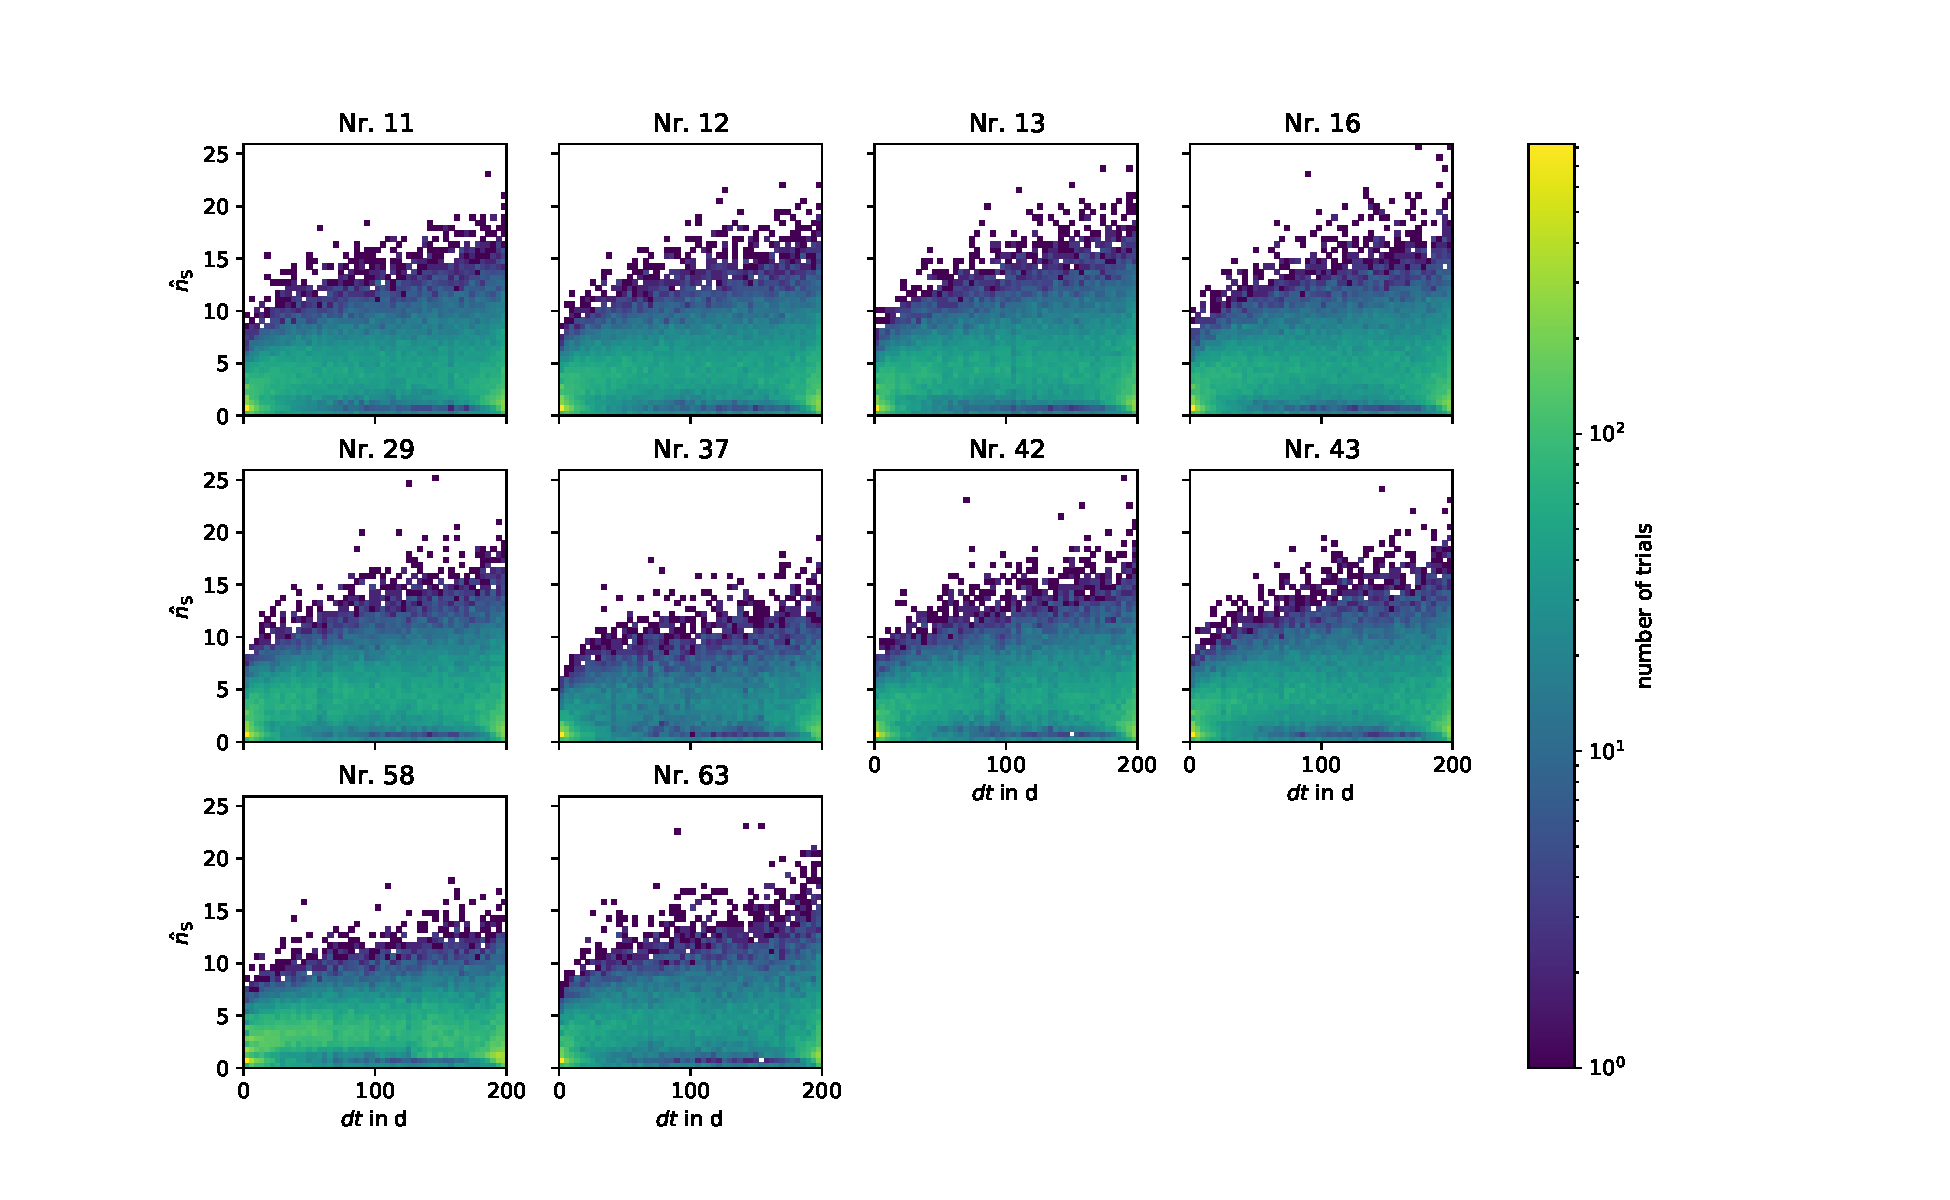
\includegraphics[width=\linewidth]{Plots/appendix/time_window_ns_sens_time_dep.pdf}
    \caption{Histograms of the time window lengths $dt$ in days in dependence of the fitted signal parameter $\hat{n}_\text{S}$ of all $\num{10}$ sources for the time-dependent analysis for the set of signal trials with the number of injected signal events closest to satisfying the condition to calculate the sensitivity.}
    \label{fig:sens_ns_dt_all}
\end{figure}

\begin{figure}
    \centering
    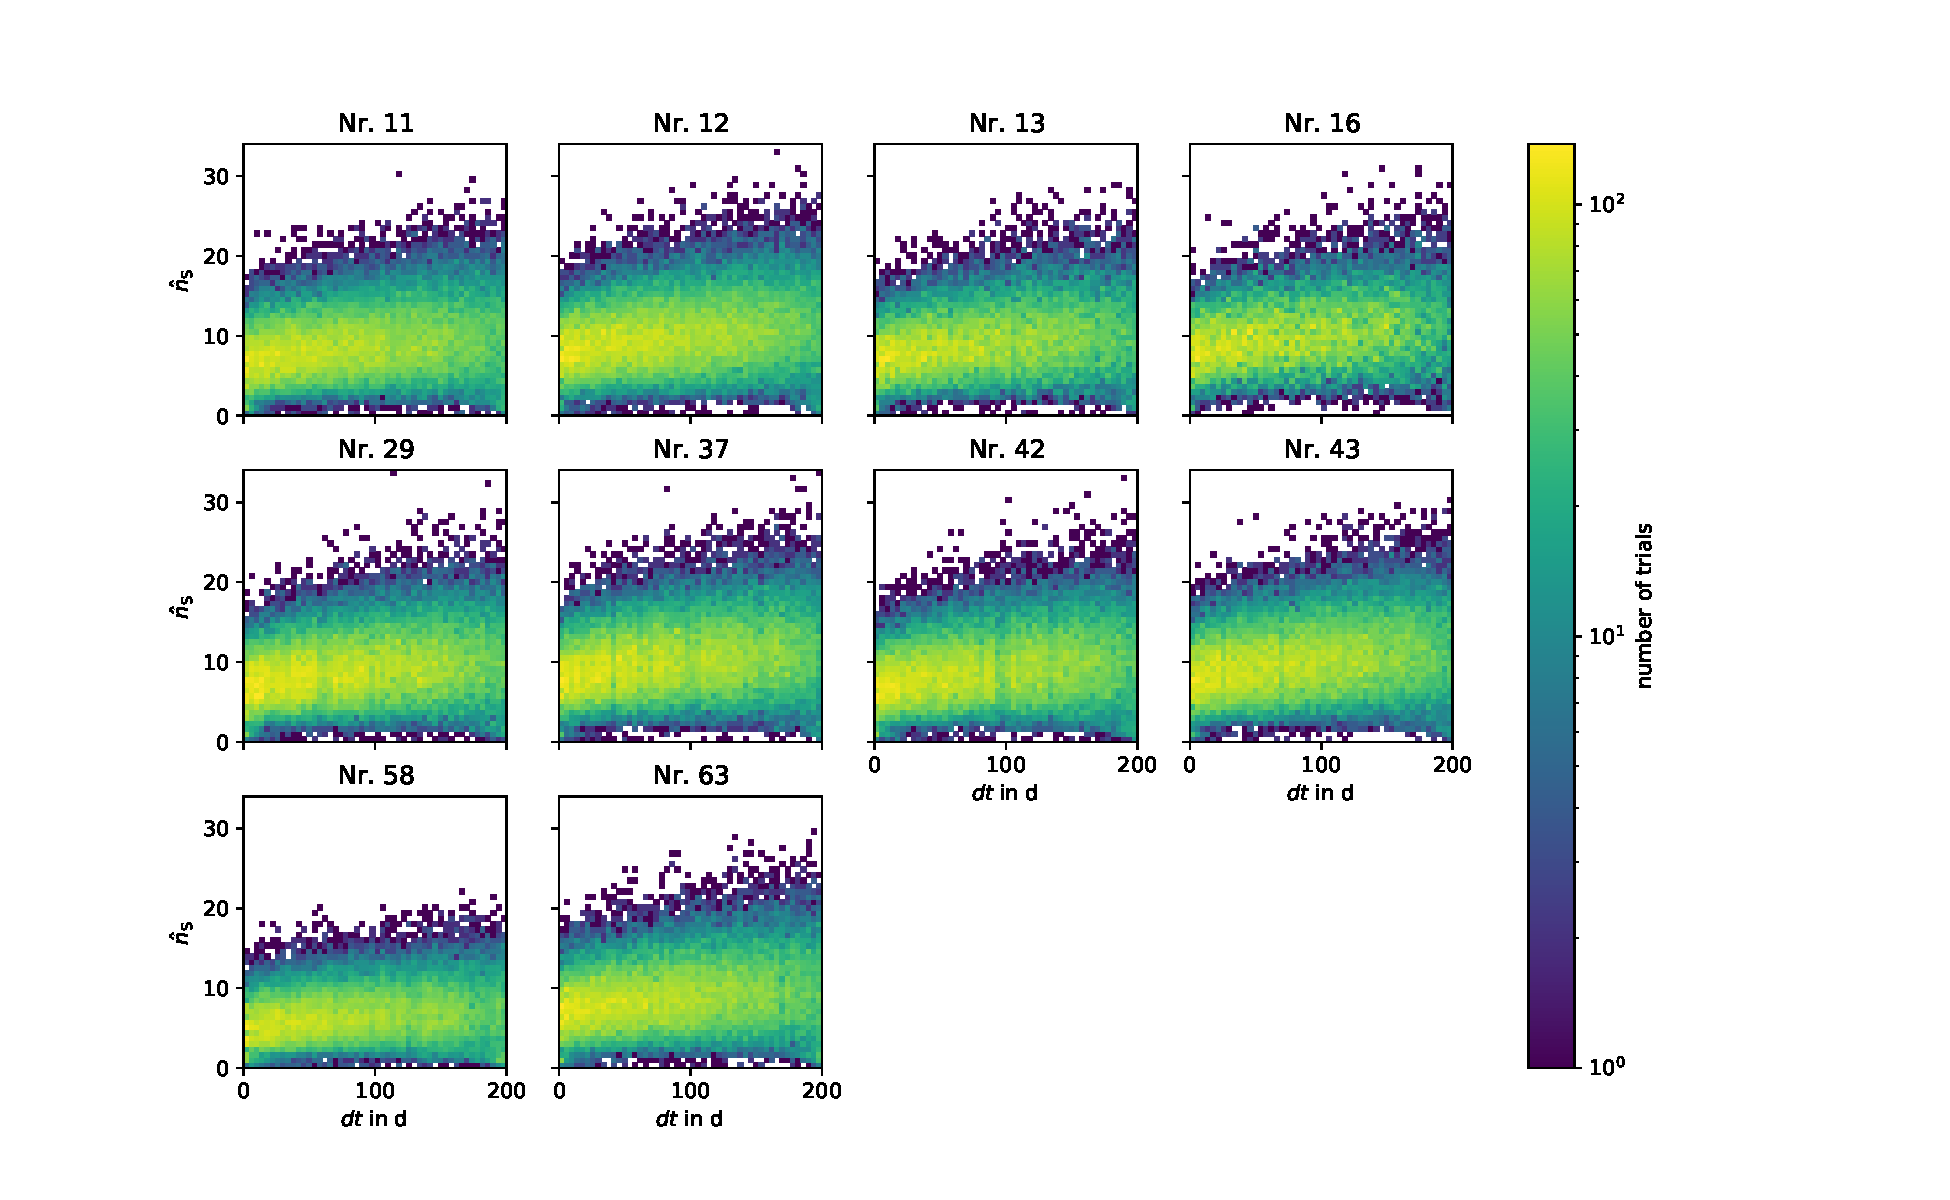
\includegraphics[width=\linewidth]{Plots/appendix/time_window_ns_disc_time_dep.pdf}
    \caption{Histograms of the time window lengths $dt$ in days in dependence of the fitted signal parameter $\hat{n}_\text{S}$ of all $\num{10}$ sources for the time-dependent analysis for the set of signal trials with the number of injected signal events closest to satisfying the condition to calculate the discovery potential.}
    \label{fig:disc_ns_dt_all}
\end{figure}

\newpage
\subsection{Examination of Fit Bias} \label{sec:fit_bias_time_dep}

\begin{figure}
    \centering
    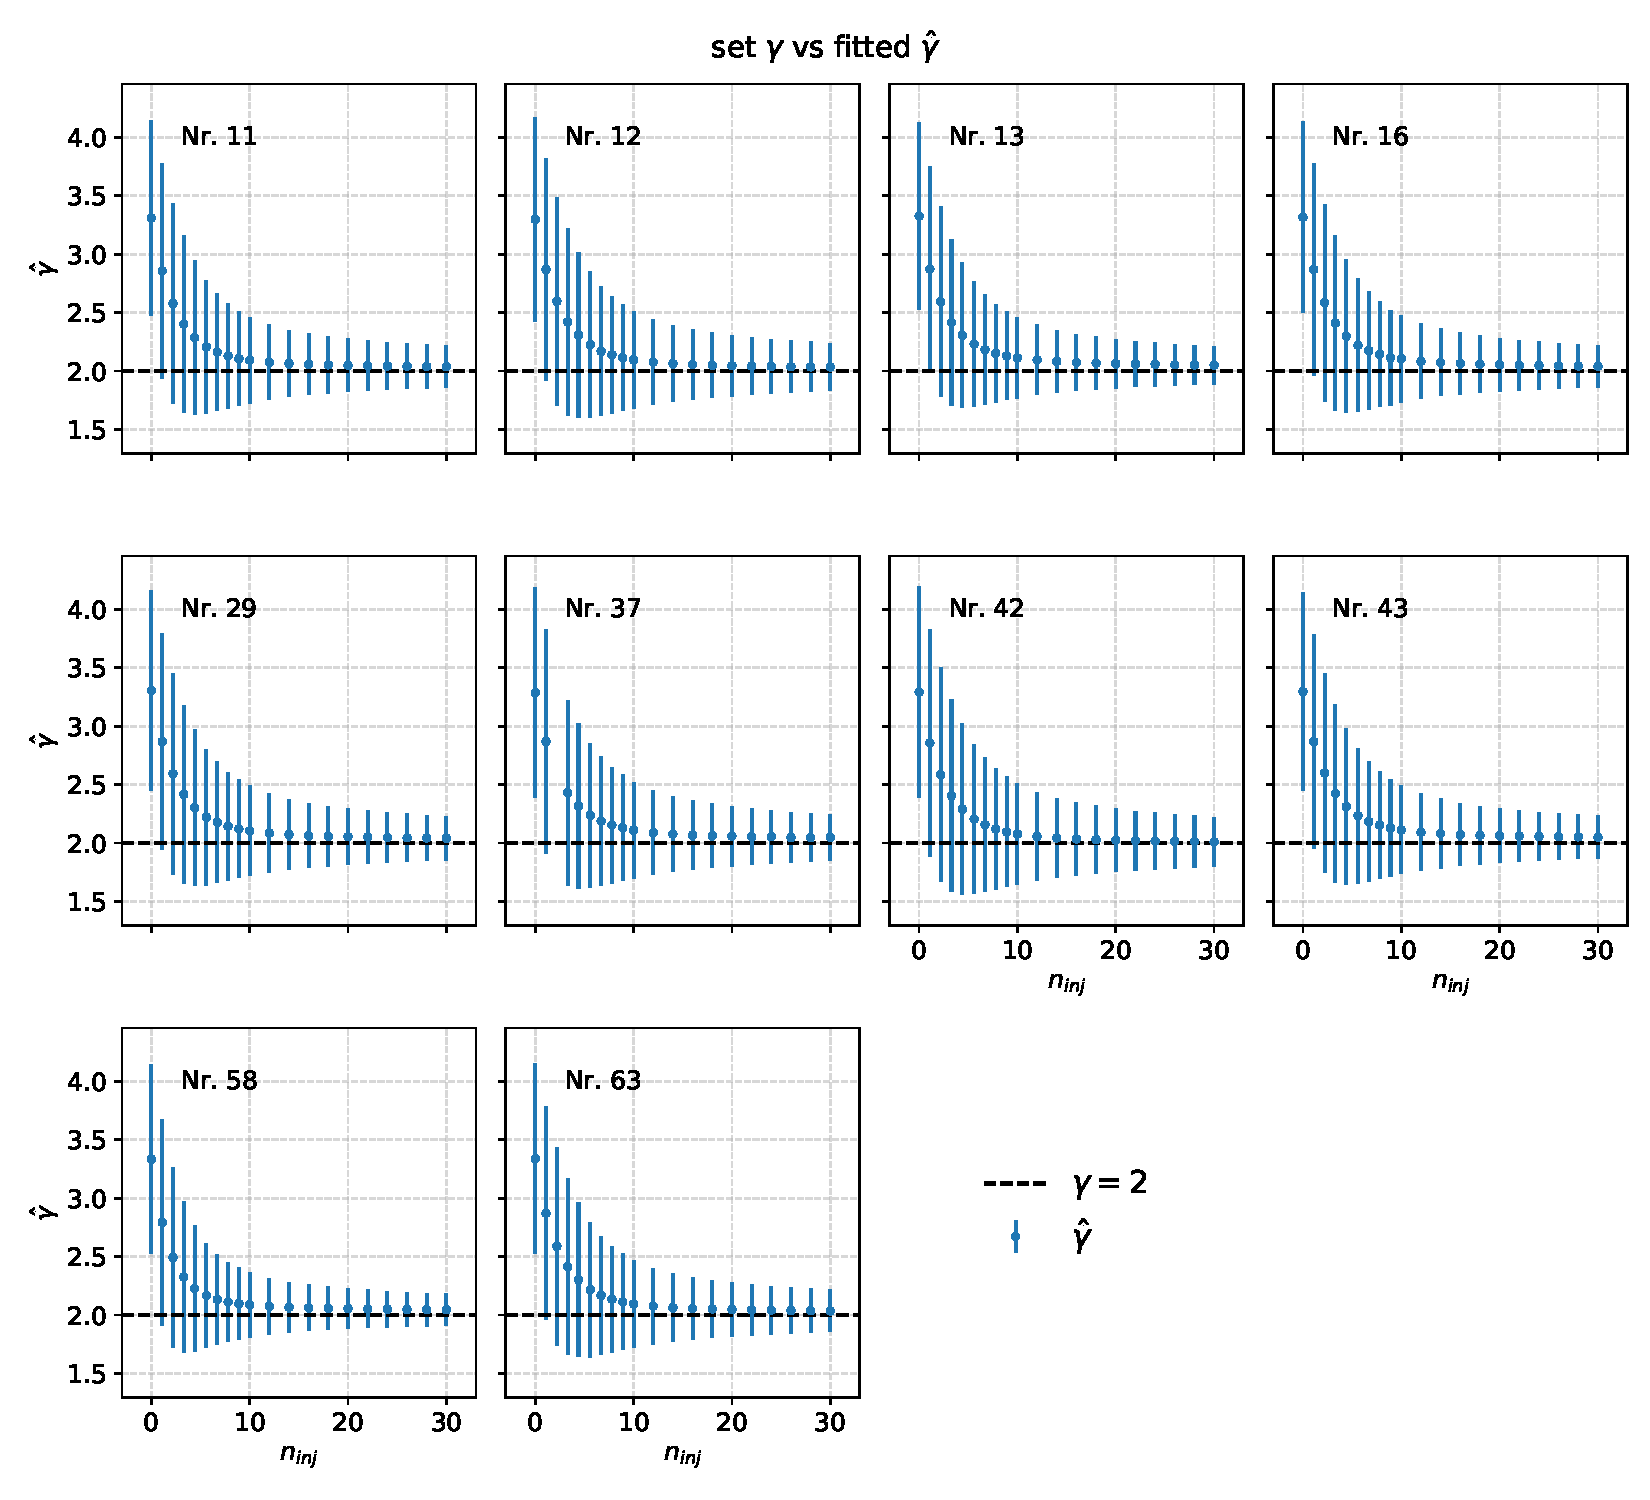
\includegraphics[width=\linewidth]{Plots/appendix/gamma_fit_time_dep.pdf}
    \caption{Fitted spectral index $\hat\gamma$ in dependence of the injected number of signal events $n_\text{inj}$ with spectral index $\gamma$, shown with a horizontal black dashed line, for the trials used in the time-dependent analysis.}
    \label{fig:gamma_fit_time_dep}
\end{figure}

\begin{figure}
    \centering
    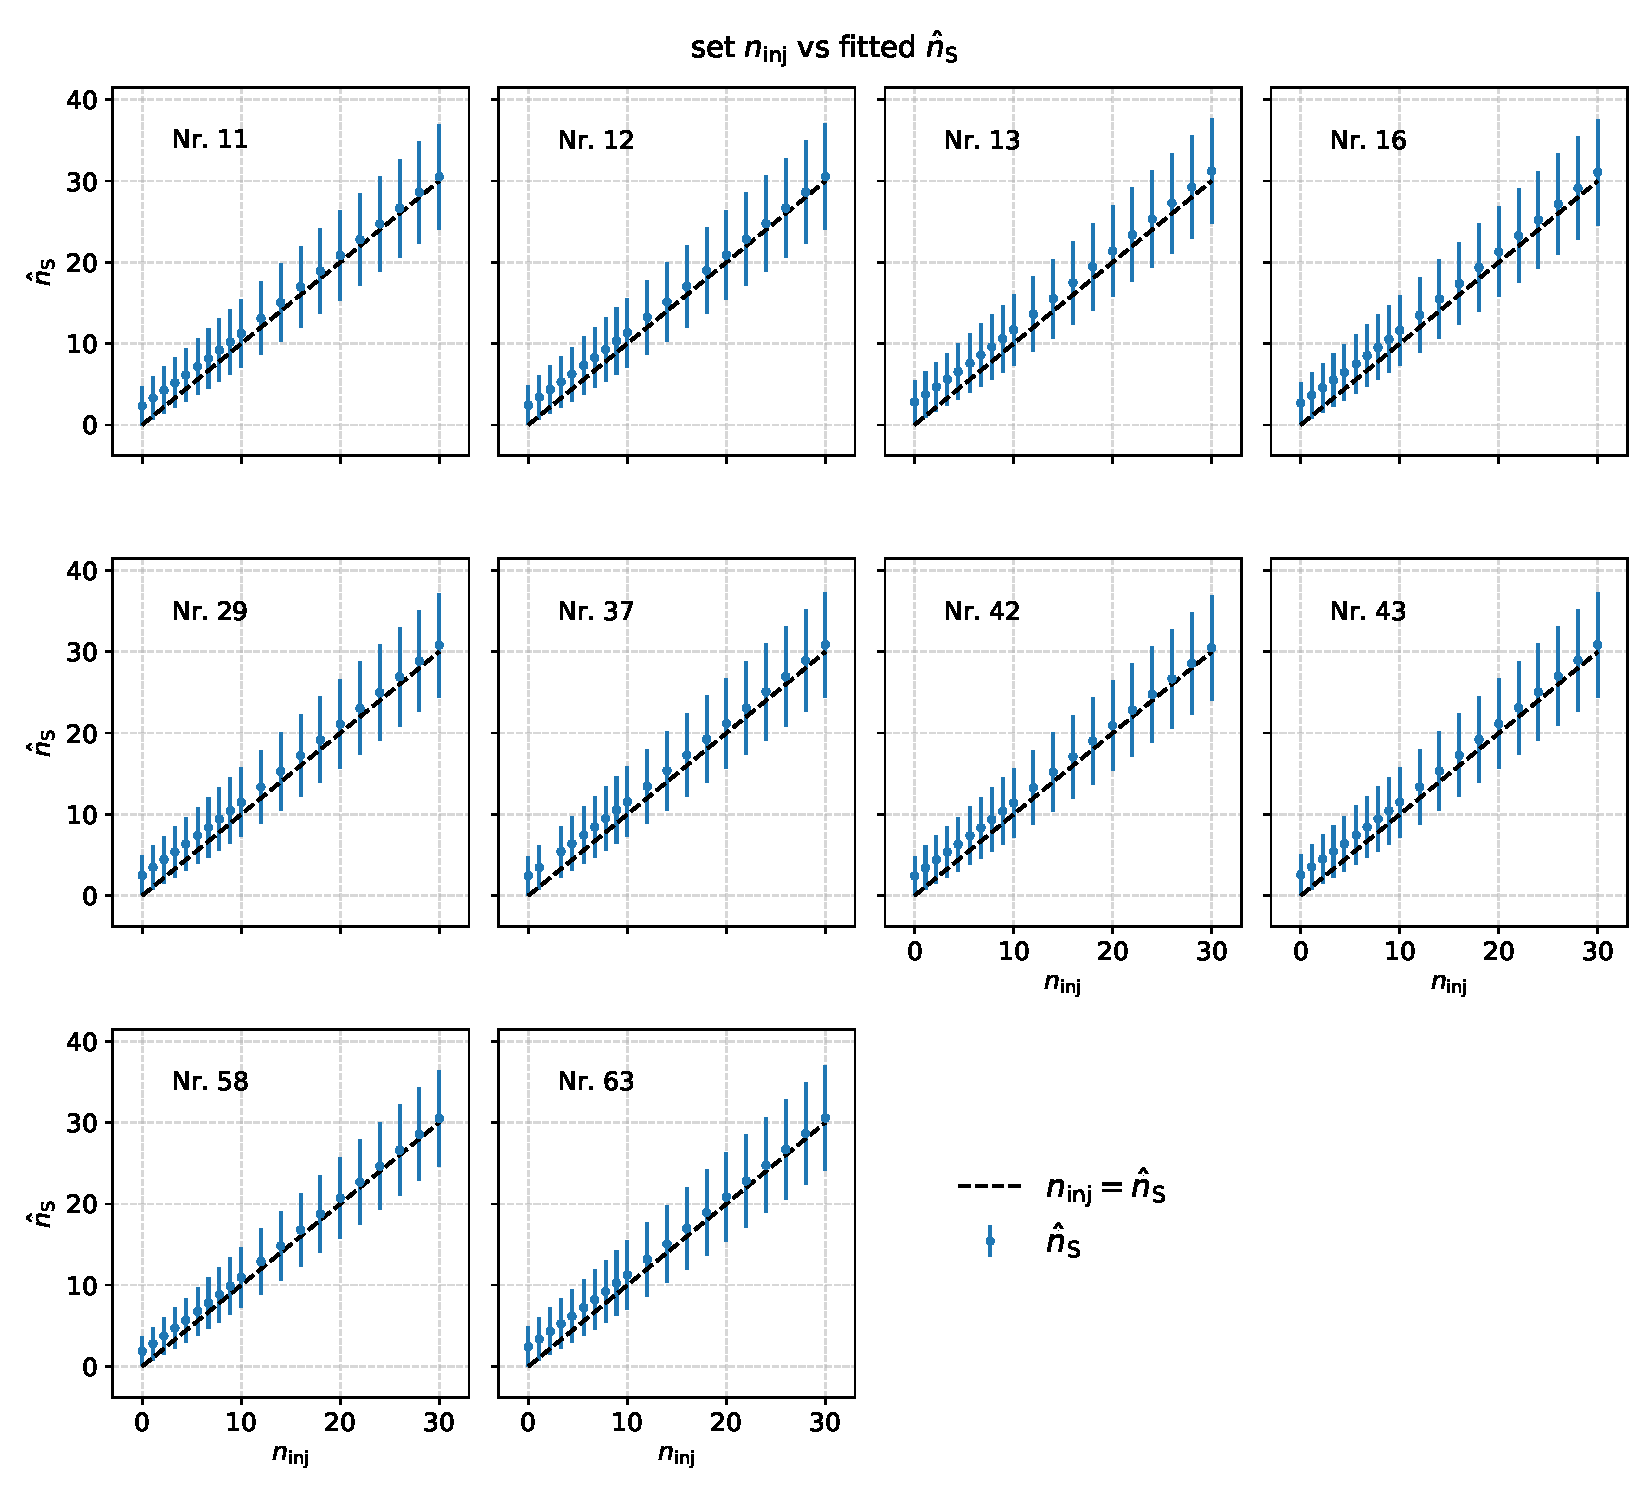
\includegraphics[width=\linewidth]{Plots/appendix/ns_fit_time_dep.pdf}
    \caption{Fitted number of signal events $\hat{n}_{\text{S}}$ in dependence of the injected number of signal events $n_\text{inj}$ with spectral index $\gamma$ for the time-dependent analysis. The black dashed line shows the equality of the fitted and the injected number of signal events.}
    \label{fig:ns_fit_time_dep}
\end{figure}

\section{Conclusion and Outlook}

This chapter contains the figure for the attempted trial correction.
Adding this into the main part would hurt the reading flow too much, thus its positioning here.

\begin{figure}
    \centering
    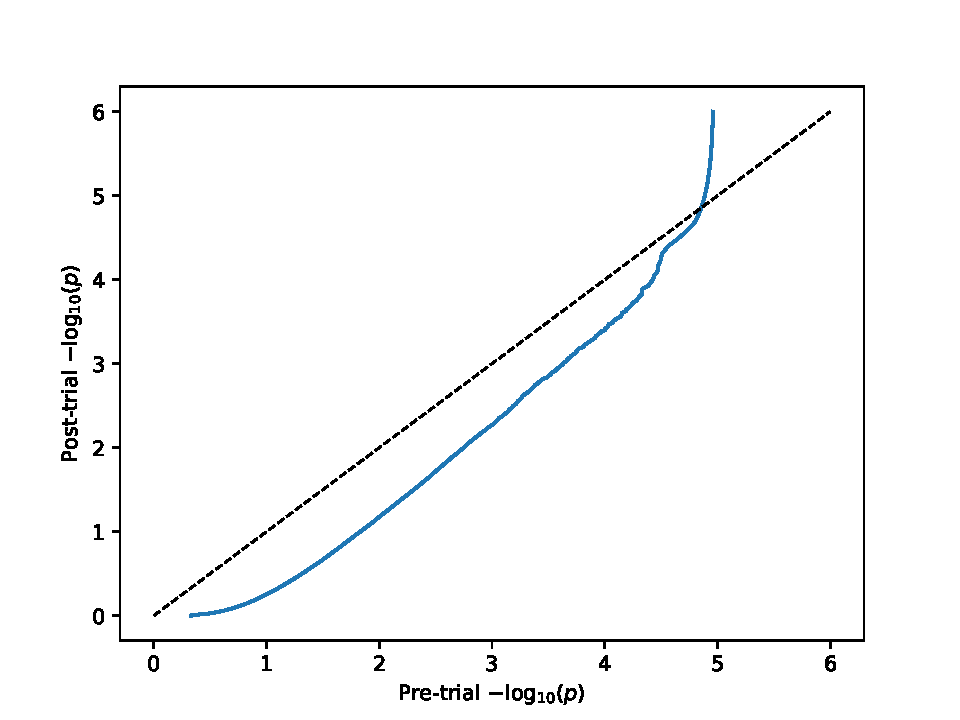
\includegraphics[width=\linewidth]{Plots/appendix/post_trial_p_values_1.pdf}
    \caption{Attempted trial correction for the time-dependent analysis. Normally the incline of the blue line should not be greater than the incline of the diagonal dashed line.}
    \label{fig:post_trials}
\end{figure}

\chapter{Reproduction}

This chapter contains all the necessary information to reproduce the analyses.

\section{Main Analyses}

The analysis repo can be found at \url{https://github.com/cybajohn/csky_gfu_stacking}.
The analysis was written on the external server cobalt and is located at
\begin{verbatim}
          /home/jkollek/punktquellensuche/csky_ehe_stacking.
\end{verbatim}
It was written in \texttt{Python3} version 3.7.5 and uses \texttt{csky} version 1.1.7.
To compile it, the shell under
\begin{verbatim}
          /home/jkollek/venvs/py3v4/bin/python
\end{verbatim}
was used.
This shell contains all the necessary dependencies to run the analysis.
In order to be able to reproduce the analysis, the directories in the \texttt{\_paths.py} file must first be adapted to the user.
The analysis should be done in three main steps, the data preparation, the time-integrated analysis and the time-dependent analysis.

\subsection{Data Preparation}
The first step is to create the source files for the neutrino sources through the \texttt{make\_source\_files\_from\_fits.py} file.
The skymaps are created by the file \texttt{make\_skymap.py}.
This is followed by the creation of the preprocessed datasets.
The script \texttt{check\_gold\_filter\_jobs.py} creates job files that can be processed on the server condor, these use the script \texttt{check\_gold\_mc\_ids.py} and can be started in the job folder with the bash command on condor,\\ (here: \texttt{bash ehe\_transient\_stacking.dag.start.sh}).
Once the scripts have run, they can be collected via \texttt{check\_gold\_filter\_combine.py} and the actual prepared datasets can be created via the \texttt{remove\_gold\_from\_data.py} script.
These datasets can now be inserted into \texttt{csky} into the \texttt{selections.py} file via creating a new dataset class.

\begin{verbatim}
class my_cleaned_data(PSDataSpec):
    _user_path = os.path.join("/data","user","jkollek",
                              "csky_ehe_stacking","rawout_tests",
                              "cleaned_datasets_new")
    _path_sig = os.path.join(_user_path,'IC86_2016_MC.npy')
    _path_data = [os.path.join(_user_path,'IC86_2011_exp.npy'),
                  os.path.join(_user_path,'IC86_2012_exp.npy'),
                  os.path.join(_user_path,'IC86_2013_exp.npy'),
                  os.path.join(_user_path,'IC86_2014_exp.npy'),
                  os.path.join(_user_path,'IC86_2015_exp.npy'),
                  os.path.join(_user_path,'IC86_2016_exp.npy'),
                  os.path.join(_user_path,'IC86_2017_exp.npy'),
                  os.path.join(_user_path,'IC86_2018_exp.npy'),
                  os.path.join(_user_path,'IC86_2019_exp.npy')]
    _path_grls = [os.path.join(_user_path,'GRL','IC86_2011_exp.npy'),
                  os.path.join(_user_path,'GRL','IC86_2012_exp.npy'),
                  os.path.join(_user_path,'GRL','IC86_2013_exp.npy'),
                  os.path.join(_user_path,'GRL','IC86_2014_exp.npy'),
                  os.path.join(_user_path,'GRL','IC86_2015_exp.npy'),
                  os.path.join(_user_path,'GRL','IC86_2016_exp.npy'),
                  os.path.join(_user_path,'GRL','IC86_2017_exp.npy'),
                  os.path.join(_user_path,'GRL','IC86_2018_exp.npy'),
                  os.path.join(_user_path,'GRL','IC86_2019_exp.npy')]
    _bins_sindec = np.unique(np.concatenate([
                        np.linspace(-1, -0.93, 4 + 1),
                        np.linspace(-0.93, -0.3, 10 + 1),
                        np.linspace(-0.3, 0.05, 9 + 1),
                        np.linspace(0.05, 1, 18 + 1) ]) )
    _bins_logenergy = np.arange(1, 9.5 + 0.01, 0.125)
\end{verbatim}

\subsection{Time-Integrated Analysis}

Both analyses are basically structured in the same way.
First, the background trials are calculated and then the signal trials.
Before the actual background trials, the trials can be tested with the help of the \texttt{bg\_trial.py} script.
This is a simple setup to see how the trials work.
However, this script is not required for the analysis.
The analysis starts with the \texttt{bg\_trial\_jobs.py} script, which as before creates jobfiles for use on condor.
As before, these are collected via the \texttt{bg\_trial\_combine.py} script.
The signal trials have the same structure.

\subsection{Time-Dependent Analysis}

The same procedure as before applies here, the time-dependent scripts are identified by the \texttt{\_time\_dependent} suffix.
The post-trials can be executed via the \texttt{post\_trial*} scripts.
The scripts with the \texttt{inspect*} prefix are used to create additional plots and provide extra insight into the quantitative content of the analyses.

\section{Time-Dependent Stacking Software Approach}

The repository for the attempted analysis can be found at \url{https://github.com/cybajohn/ehe_transient_stacking_analysis_tests} and the modified \texttt{tdepps} software at \url{https://github.com/cybajohn/tdepps}.
The order of the scripts can be inferred from their name, other than that, technicalities like adjusting path names need to be done first as explained in the other analyses.
This analysis repository was formed by the constant tests of the performance of the new \texttt{tdepps} software and is therefore unfortunately not so clearly comprehensible.
An important point worth mentioning is that the analysis parameters can be adjusted in the script.

%\chapter{Acknowledgements}
%
%This thesis took me a long time and it would not have been possible for me to perform the work or finish it without the help of many people.
%First I would like to thank prof. dr. dr. Wolfgang Rhode for the opportunity to write my thesis and both them and dr. Johannes Erdmann for grading it.
%
%Then I want to thank my inner circle consisting of dr. Jan Soedingrekso, dr. Alexander Sandrock, dr. Thorben Menne and Jean-Marco Alameddine for holding %weekly meetings with me for such a long time always keeping me motivated and helping me with all their knowledge and insights.
%
%Keeping on track with insights, I would like to thank the IceCube collaboration and more precisely the people from realtime, pont source searches and %csky for their help and cooperation in answering questions.
%
%Then of course a huge thanks also to the Prüfungsverwaltung for their good cooperation.
%
%Also I would like to mention my good friends Max Pernklau, David Müller and soonish doctor Robin Denz for proofreading this thesis and always keeping me %in high spirits.
%
%Finally a huge thanks to my family and my cat for keeping me alive and well so I could finish my studies even though you may never know how much I have %struggled with this.
